\documentclass[UTF8]{ctexart}

\usepackage{caption}
\usepackage{amsmath, amssymb}
\usepackage{geometry}
\usepackage{graphicx}
\usepackage{booktabs}
\usepackage{float}
\usepackage{caption}
\usepackage{enumitem}
\usepackage{fancyvrb}
\usepackage{subcaption}
\usepackage{tabularx}
\usepackage{fancyhdr}
\usepackage{titlesec}
\usepackage{indentfirst}
\usepackage{multirow}
\usepackage{colortbl}
\usepackage{xcolor}
\definecolor{headcolor}{RGB}{70, 130, 180}    % 钢蓝色表头
\definecolor{rowcolor1}{RGB}{240, 248, 255}   % 极浅蓝色奇数行
\definecolor{rowcolor2}{RGB}{255, 255, 255}   % 白色偶数行
\usepackage[table]{xcolor}

\definecolor{headcolor}{RGB}{70, 130, 180}
\definecolor{rowcolor1}{RGB}{240, 248, 255}
\definecolor{rowcolor2}{RGB}{255, 255, 255}

\setcounter{secnumdepth}{4}
\setcounter{tocdepth}{4}

\setcounter{secnumdepth}{4}
\setcounter{tocdepth}{4}

\usepackage{titlesec}

\setcounter{secnumdepth}{4}

\titleformat{\paragraph}[hang]
  {\normalfont\normalsize\bfseries}
  {\theparagraph}{1em}{}
\titlespacing*{\paragraph}
  {0pt}{3.25ex plus 1ex minus .2ex}{1em}

\renewcommand\theparagraph{\thesubsubsection.\arabic{paragraph}}
\usepackage{listings}
\lstset{
    basicstyle=\footnotesize\ttfamily,
    breaklines=true,
    breakindent=0pt,
    numbers=left,
    numberstyle=\tiny,
    showstringspaces=false,
    frame=single,
    xleftmargin=8pt,
    xrightmargin=8pt,
    columns=fullflexible
}

% 设置纸张和页边距
\geometry{top=2.54cm, bottom=2.54cm, left=3.17cm, right=3.17cm}

% 设置页码
\pagestyle{fancy}
\fancyhf{}
\fancyfoot[C]{\thepage}
\renewcommand{\headrulewidth}{0pt}

% 设置标题格式
\titleformat{\section}{\centering\zihao{4}\bfseries}{\thesection\quad}{0pt}{}
\titleformat{\subsection}{\zihao{-4}\bfseries}{\thesubsection\quad}{0pt}{}
\titleformat{\subsubsection}{\zihao{-4}\bfseries}{\thesubsubsection\quad}{0pt}{}

% 设置全文基本字体：小四号宋体，行距1.3倍
\renewcommand{\baselinestretch}{1.3}
\zihao{-4}

% 设置论文题目
\makeatletter
\renewcommand{\maketitle}{
    \begin{center}
        {\zihao{3}\bfseries\@title}
        \vskip 1em
        {\@author}
        \vskip 1em
        {\@date}
    \end{center}
}
\makeatother

\setlength{\parindent}{2em}

% 重新定义摘要环境
\renewenvironment{abstract}
{
    \par
    \begin{center}
        {\Large\bfseries 摘要}
    \end{center}
    \par\vspace{0.5em}
    \normalsize
}
{
    \par
}

\title{基于热湿耦合与径向收缩模型的药材烘干过程研究}
\author{}
\date{}

\begin{document}

\maketitle

\begin{abstract}
\normalsize


\textbf{针对问题一}，考虑药材为长圆柱，轴向尺寸远大于半径，且半径固定，因此本文将烘干初期的传热传质过程简化为固定半径的一维径向模型。热量由表面向中心传导，水分由内部向表面扩散；问题一中热物性为常数，水分扩散系数仅随水分浓度变化，温度场与水分场之间无直接双向耦合项，故二者分别求解。分别建立热传导方程与非线性扩散方程，表面采用对流换热与对流传质的Robin（第三类）边界条件，中心取对称边界，烘房温湿度由附件1插值作为时变驱动量。空间采用有限体积法离散，时间用自适应隐式BDF推进，得到1800s内药材温度与水分浓度的时空分布，并输出指定时刻与位置的结果。

\textbf{针对问题二}，

\textbf{针对问题三}，

\textbf{针对问题四}，

最后，

\vspace{0.5cm}
\noindent\textbf{关键词：} 
\end{abstract}

\newpage

\section{问题重述}

\subsection{问题背景与研究对象}

热风干燥是中药材加工中的常用工序，通常包括预热平衡和恒温干燥两个阶段。烘房温湿环境影响药材的升温与失水过程，因此需要描述内部温度和含水率的时空变化，为判断干燥进程与结束时间提供依据。

本文研究对象为长 \(25~\mathrm{cm}\)、初始半径 \(2~\mathrm{cm}\) 的圆柱形药材，初始温度为 \(28~^\circ\mathrm{C}\)，初始干基含水率为 \(2.55~\mathrm{kg/kg}\)。附件1、2分别提供烘房温度及水分浓度、药材半径随时间的变化数据，题目附录2--4给出各问所用的物性参数与经验公式。

\subsection{问题提出}

根据上述条件，需要建立数学模型解决以下四个问题：

\textbf{问题一：预热阶段的温湿分布。}依据题目附录2参数，建立预热平衡阶段温度与含水率变化模型，计算前 \(1800~\mathrm{s}\) 内的分布，并给出指定时刻与径向位置的结果。

\textbf{问题二：变物性条件下的温湿演化。}统一采用题目附录3经验公式，建立适用于整个烘干过程的温度与含水率变化模型，给出前 \(3~\mathrm{h}\) 每隔 \(0.5~\mathrm{h}\) 的规定位置结果。

\textbf{问题三：全域达标所需时间。}在问题二所述条件下，确定药材各处含水率均低于 \(0.15~\mathrm{kg/kg}\) 所需的烘干时间，并给出每隔 \(6~\mathrm{h}\) 及烘干结束时的径向含水率。

\textbf{问题四：考虑尺寸收缩的烘干时长。}结合附件2的半径变化与题目附录4经验公式，考虑药材收缩，重新确定全域达标时间，并给出每隔 \(6~\mathrm{h}\) 及结束时内部规定位置与当前表面的含水率。



\section{问题分析}

\subsection{问题一的分析}

预热过程中，热量从药材表面传向内部，水分则由内部向表面迁移，因而需要同时关注时间变化和内部位置差异。首先，对附件1的离散数据作分段线性插值，得到任意时刻的烘房温度和水分浓度，作为分析药材变化的外部条件。然后，结合圆柱形状以及计算结果，确认端面影响可忽略，因此沿半径方向考察传热与失水。由附录2可知，温度变化不影响水分扩散，含水率变化也不改变热物性，因此可分别求解两个过程。最后采用有限体积法获得温度和含水率的时空分布，从中提取指定结果，并比较表面与中心的变化。

\subsection{问题二的分析}

第二问统一采用附录3的经验关系，需先梳理物性与温度、含水率之间的联系。含水率变化会影响药材的吸热和导热能力，而温度变化又会影响水分扩散，说明两者需要在计算过程中相互反馈。因此，沿用第一问对环境和径向传输过程的处理，从题设初态重新计算，在求解温度与含水率的同时更新各处物性，得到前 \(3~\mathrm{h}\) 的温湿分布。在此基础上，比较不同位置的升温与失水过程，再结合扩散系数的变化，分析升温促进扩散与含水率降低抑制扩散的共同作用。

\subsection{问题三的分析}

药材各处均达标，取决于最湿位置何时满足要求。因此，先从每一时刻的径向分布中确定最大含水率，将全域达标要求转化为该最大值首次降至阈值的时间判定。为获得完整的变化过程，需延长第二问的计算；而附件1的环境记录仅到 \(4~\mathrm{h}\)，故在后续环境保持稳定的假设下，以观测末段的平均水平向后延拓，继续联合计算温度与含水率。随后，找出最大含水率跨越 \(0.15~\mathrm{kg/kg}\) 的时间区间，在区间内细化求解，确定临界时刻，并继续计算确认各处均严格低于阈值。由此得到烘干时间及规定时刻的径向含水率分布。

\subsection{问题四的分析}

考虑收缩后，药材内部材料及表面的位置不断变化，首先需对附件2的半径数据作插值，得到各时刻的药材尺寸。为持续跟踪同一部分材料，在长度不变、径向同比收缩的假设下，可用其相对于当前半径的位置表示所在部位，使不同时刻的计算位置相互对应。据此更新传输距离与表面位置，采用附录4物性从题设初态重新计算，并按第三问的判定思路求出烘干时间。再将相对位置换回实际距离，提取规定位置与当前表面的含水率。



\section{模型假设}


\begin{enumerate}
\item 药材为长圆柱，长径比远大于 \(1\)，忽略两端端面的轴向效应，仅考虑半径方向的一维径向传热传质；
\item 在预热平衡阶段（\(0\sim1800\mathrm{s}\)），药材半径固定为 \(2\mathrm{cm}\)，不随时间变化；
\item 热物性参数取题目附录2给出的常数，不随温度和含水率变化；
\item 水分扩散系数仅随含水率变化，不随温度变化；
\item 温度场与水分场之间无直接双向耦合项，二者可分别求解；
\item 不额外加入蒸发潜热和内部热湿耦合效应，这是题目未给出相变参数情况下的建模取舍。
\end{enumerate}


\section{符号说明}



\section{模型准备}

\subsection{问题背景}

中药材热风烘干是热量与水分同时向药材内部和外部传递的过程：热空气通过对流换热把热量传给药材表面，再依靠温度梯度向中心传导；表面水分向环境蒸发，内部水分在浓度梯度驱动下向表面扩散补充。由于药材内部同时存在温度梯度和水分浓度梯度，这是一个典型的传热与传质耦合问题。

本文所研究的药材为圆柱形，长 \(25\mathrm{cm}\)、半径 \(2\mathrm{cm}\)，长径比达到 \(12.5\)，远大于 \(1\)。在烘干初期，两端端面的散热和失水面积与侧面相比很小，药材内部的温度和水分浓度沿半径方向的变化远大于沿轴向的变化。因此，本文将三维问题简化为以中心轴为对称轴的一维径向传热传质问题。

\subsection{传热传质的基本方式}

热量传递主要有三种方式：热传导、对流和辐射。本文研究的热量在药材内部主要靠热传导传递。傅里叶定律指出，单位时间内通过单位面积的热量，与温度沿传递方向的变化率成正比，方向从高温指向低温，即
\begin{equation}
q=-k\frac{\partial T}{\partial r},
\end{equation}
其中 \(q\) 为热流密度（\(\mathrm{W/m^2}\)），\(k\) 为导热系数（\(\mathrm{W/(m\cdot K)}\)），负号表示热量从高温流向低温。

水分在药材内部的迁移规律与热传导类似，但驱动力为水分浓度梯度。菲克扩散定律指出，单位时间内通过单位面积的水分量，与水分浓度沿传递方向的变化率成正比，即
\begin{equation}
J=-D\frac{\partial C}{\partial r},
\end{equation}
其中 \(J\) 为水分通量，\(D\) 为水分扩散系数，\(C\) 为干基含水率。

本文在预热平衡阶段（\(0\sim1800\mathrm{s}\)）中，题目给出的热物性均为常数，水分扩散系数仅随含水率变化，且温度场与水分场之间无直接双向耦合项，因此温度场与水分场可分开求解。后续问题中物性将随含水率变化、水分扩散系数同时依赖温度和含水率，温度场与水分场需要联立推进。

\subsection{边界条件类型}

导热问题常见边界条件有三类。令 \(T(r,t)\) 为温度分布函数，\(\Gamma\) 为边界曲面。

第一类边界条件规定边界上的温度值：
\begin{equation}
T(r,t)\big|_{r\in\Gamma}=f(r,t).
\end{equation}
第二类边界条件规定边界上的热流密度：
\begin{equation}
\frac{\partial T}{\partial n}\bigg|_{r\in\Gamma}=f(r,t).
\end{equation}
第三类边界条件规定边界上物体与周围流体间的对流传热系数及周围流体温度：
\begin{equation}
\left(\frac{\partial T}{\partial n}+\sigma T\right)\bigg|_{r\in\Gamma}=f(r,t).
\end{equation}
本文药材表面与烘房热空气直接接触，热量和水分均通过表面进出，采用第三类边界条件（Robin 边界）。

\subsection{几何简化与坐标建立}

药材为长圆柱，半径 \(R=0.02~\mathrm{m}\)，长度 \(L=0.25~\mathrm{m}\)，端面面积与侧面积之比为
\begin{equation}
\frac{S_{\mathrm{ends}}}{S_R}=\frac{R}{L}=\frac{0.02}{0.25}=0.08.
\end{equation}
端面交换远小于侧面交换，故忽略轴向梯度和端面交换，仅考虑 \(0\le r\le R\) 的一维径向问题。

建立以药材中心轴为对称轴、半径方向为 \(r\) 轴的径向坐标。热量沿半径方向由表面向中心传导，水分由内部向表面扩散。

\begin{figure}[H]
\centering
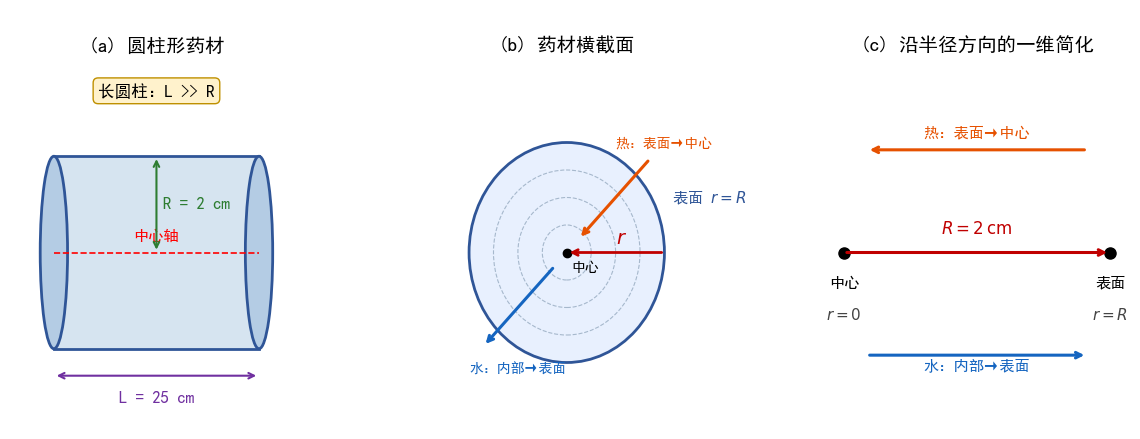
\includegraphics[width=0.95\textwidth]{fig1.png}
\caption{圆柱形药材简化示意图}
\label{fig:radial_simplification}
\end{figure}

如图~\ref{fig:radial_simplification} 所示，药材可视为长圆柱，热量沿半径方向由表面向中心传导，水分则由内部向表面扩散；由于长径比远大于 \(1\)，本文将三维圆柱问题简化为以中心轴为对称轴的一维径向问题。

\subsection{各物理环节的传热传质方式}

药材表面直接与烘房热空气接触，热量和水分均通过表面进出药材。

热量方面，热空气通过对流换热将热量传给药材表面，边界条件为
\begin{equation}
-k\frac{\partial T}{\partial r}\bigg|_{r=R}=h\left[T(R,t)-T_\infty(t)\right],
\label{eq:bcT}
\end{equation}
其中 \(h\) 为对流换热系数，\(T_\infty(t)\) 为烘房空气温度。

水分方面，药材表面的水分通过对流传质进入烘房空气，边界条件为
\begin{equation}
-D(C_s)\frac{\partial C}{\partial r}\bigg|_{r=R}=h_m\left[C_s-C_e(t)\right],
\label{eq:bcC}
\end{equation}
其中 \(h_m\) 为对流传质系数，\(C_s\) 为表面含水率，\(C_e(t)\) 为环境水分驱动量。由于题目未给出空气湿度与药材含水率之间的严格换算关系，本文将附件 1 给出的环境水分量直接作为表面传质的等效驱动量使用。

初始时刻药材温度均匀为 \(28^\circ\mathrm{C}\)，含水率均匀为 \(2.55\mathrm{kg/kg}\)，即
\begin{equation}
T(r,0)=28,\qquad C(r,0)=2.55.
\label{eq:ic}
\end{equation}
药材中心处由于几何对称，径向不存在净传递，取对称边界条件
\begin{equation}
\frac{\partial T}{\partial r}(0,t)=0,\qquad \frac{\partial C}{\partial r}(0,t)=0.
\label{eq:sym}
\end{equation}

\subsection{符号说明}

\begin{table}[H]
\centering
\caption{主要变量与符号}
\label{tab:symbols}
\begin{tabularx}{\textwidth}{|>{\centering\arraybackslash}p{3cm}|>{\centering\arraybackslash}X|>{\centering\arraybackslash}p{3.5cm}|}
\hline
\rowcolor{headcolor}
\textbf{符号} & \textbf{含义} & \textbf{单位} \\
\hline
\rowcolor{rowcolor1}
\(r\)、\(t\) & 距圆柱轴线的距离、烘干时间 & m、s \\
\hline
\rowcolor{rowcolor2}
\(T\)、\(T_K\) & 摄氏温度、绝对温度 & \(^\circ\mathrm{C}\)、K \\
\hline
\rowcolor{rowcolor1}
\(C\) & 干基含水率 & kg/kg \\
\hline
\rowcolor{rowcolor2}
\(\rho\)、\(c_p\) & 密度、比热容 & kg/m\(^3\)、J/(kg·K) \\
\hline
\rowcolor{rowcolor1}
\(k\)、\(D\) & 导热系数、有效水分扩散系数 & W/(m·K)、m\(^2\)/s \\
\hline
\rowcolor{rowcolor2}
\(h\)、\(h_m\) & 表面换热系数、有效传质系数 & W/(m\(^2\)·K)、m/s \\
\hline
\rowcolor{rowcolor1}
\(T_\infty\)、\(C_e\) & 环境温度、有效环境水分驱动量 & \(^\circ\mathrm{C}\)、kg/kg \\
\hline
\end{tabularx}
\end{table}

\section{问题一模型的建立与求解}

\subsection{问题一分析}

问题一研究预热平衡阶段（\(0\sim1800\mathrm{s}\)）的温度场与水分浓度场。该阶段热物性均为常数，水分扩散系数仅随含水率变化，温度场与水分场之间无直接双向耦合项，二者可分别建立方程并独立求解。这是问题一区别于后续问题的关键假设，也是本文选择分开求解的依据。

\subsection{模型建立}

\subsubsection{控制方程}

根据模型准备，药材内部温度场满足圆柱坐标下的热传导方程

\subsubsection{定解条件}

初始条件为
\begin{equation}
T(r,0)=28^\circ\mathrm{C},\qquad C(r,0)=2.55\mathrm{kg/kg}.
\end{equation}
中心对称边界为
\begin{equation}
\frac{\partial T}{\partial r}(0,t)=0,\qquad \frac{\partial C}{\partial r}(0,t)=0.
\end{equation}
表面第三类边界为
\begin{equation}
-k\frac{\partial T}{\partial r}(R,t)=h\left[T(R,t)-T_\infty(t)\right],
\end{equation}
\begin{equation}
-D(C_s)\frac{\partial C}{\partial r}(R,t)=h_m\left[C_s-C_e(t)\right],
\end{equation}
其中 \(T_\infty(t)\)、\(C_e(t)\) 由附件 1 的离散数据经分段线性插值得到。

\subsubsection{量级分析}

在求解前，先对问题的物理尺度作量级判断。热扩散系数为
\begin{equation}
\alpha=\frac{k}{\rho c_p}=\frac{0.36}{820\times2600}\approx1.69\times10^{-7}\,\mathrm{m^2/s},
\end{equation}
初始含水率对应的水分扩散系数为
\begin{equation}
D_0=7\times10^{-9}e^{-0.89/2.55}\approx4.94\times10^{-9}\,\mathrm{m^2/s}.
\end{equation}
由此可得热扩散特征时间
\begin{equation}
\frac{R^2}{\alpha}\approx2369\,\mathrm{s}\approx39.5\,\mathrm{min},
\end{equation}
水分扩散特征时间
\begin{equation}
\frac{R^2}{D_0}\approx81010\,\mathrm{s}\approx22.5\,\mathrm{h}.
\end{equation}
两者相差约两个数量级。这表明在 \(1800\mathrm{s}\) 内，热量已能显著影响药材中心，而水分变化主要集中在表层。

\subsection{模型求解}

\subsubsection{空间离散：有限体积法}

由于药材为圆柱形，且水分扩散系数随含水率变化，本文采用有限体积法对空间进行离散。将半径 \(0\le r\le R\) 划分为 \(N\) 个区间，节点为 \(r_i=i\Delta r\)，\(\Delta r=R/N\)，节点数为 \(N+1\)，包含中心 \(r=0\) 和表面 \(r=R\)。

对第 \(i\) 个控制体，其体积和界面面积分别为
\begin{equation}
V_i=\pi\left(r_{i+1/2}^2-r_{i-1/2}^2\right),\qquad S_{i+1/2}=2\pi r_{i+1/2},
\end{equation}
其中 \(r_{i+1/2}=(r_i+r_{i+1})/2\)。对每个控制体写出“储存量变化＝内侧通量－外侧通量”的收支关系：
\begin{equation}
m_iV_i\frac{\mathrm{d}u_i}{\mathrm{d}t}=F_{i-1/2}-F_{i+1/2},
\end{equation}
其中 \(u=T\) 时 \(m=\rho c_p\)，\(u=C\) 时 \(m=1\)。相邻控制体共享同一个界面通量，全域求和后内部通量成对抵消，仅保留边界交换，离散格式具有守恒性。

中心节点 \(r=0\) 处采用对称处理，中心控制体为半径 \(\Delta r/2\) 的小圆盘，体积为 \(V_0=\pi\Delta r^2/4\)，外侧面积为 \(\pi\Delta r\)，内侧面积为零。代入收支关系可得
\begin{equation}
\frac{\mathrm{d}T_0}{\mathrm{d}t}=\frac{4\alpha(T_1-T_0)}{\Delta r^2},
\end{equation}
水分方程对应为
\begin{equation}
\frac{\mathrm{d}C_0}{\mathrm{d}t}=\frac{4\left[\Psi(C_1)-\Psi(C_0)\right]}{r_1^2},
\end{equation}
其中 \(\Psi(C)\) 为 Kirchhoff 变量。

表面节点 \(r_N=R\) 采用精确环体积 \(V_N=\pi[R^2-r_{N-1/2}^2]\)，表面通量直接进入收支方程
\begin{equation}
\rho c_pV_N\frac{\mathrm{d}T_N}{\mathrm{d}t}=g_{N-1/2}k(T_{N-1}-T_N)-F_{R,T},
\end{equation}
\begin{equation}
V_N\frac{\mathrm{d}C_N}{\mathrm{d}t}=g_{N-1/2}\left[\Psi(C_{N-1})-\Psi(C_N)\right]-F_{R,C},
\end{equation}
其中 \(g_{N-1/2}=S_{N-1/2}/\Delta r\)，表面热通量 \(F_{R,T}=2\pi Rh(T_N-T_\infty)\)，表面质通量 \(F_{R,C}=2\pi Rh_m(C_N-C_e)\)，统一取向外为正。

\subsubsection{非线性水分通量：Kirchhoff 变换}

水分方程中 \(D\) 随 \(C\) 变化，若直接在界面上取算术平均，会引入额外近似。为保留扩散系数的非线性特征，本文引入 Kirchhoff 变量
\begin{equation}
\Psi(C)=\int_0^CD(s)\,\mathrm{d}s,
\end{equation}
从而
\begin{equation}
D(C)\frac{\partial C}{\partial r}=\frac{\partial\Psi(C)}{\partial r}.
\end{equation}
界面水分通量可写为
\begin{equation}
F_{i+1/2,C}=-g_{i+1/2}\left[\Psi(C_{i+1})-\Psi(C_i)\right].
\end{equation}
由于相邻浓度接近时直接计算两个 \(\Psi\) 值再相减可能产生数值相消，实际计算中采用浓度区间积分平均的方式计算势差
\begin{equation}
\Psi(C_R)-\Psi(C_L)=(C_R-C_L)\int_0^1D\left[C_L+s(C_R-C_L)\right]\mathrm{d}s,
\end{equation}
用固定阶 Gauss 求积计算该积分。Kirchhoff 变换只是将“系数乘梯度”改写成“扩散势的梯度”，水分方程仍以 \(C\) 为未知量，整个问题并未因此变成线性问题。

\subsubsection{时间推进：自适应隐式 BDF}

空间离散后，原偏微分方程转化为一组常微分方程
\begin{equation}
\frac{\mathrm{d}u}{\mathrm{d}t}=f(t,u),
\end{equation}
其中 \(u\) 包含所有径向节点的温度或水分浓度。本文采用自适应隐式 BDF 方法进行时间推进。BDF 是一种隐式、自适应的时间积分器，能够在初期变化剧烈时自动减小内部步长，在后期变化平缓时增大步长。题目要求每 \(1\mathrm{s}\) 保存一次结果，但这只是输出间隔，并不等于 BDF 的内部步长也必须为 \(1\mathrm{s}\)。

温度和水分分别独立积分，各自采用不同的绝对容差。环境数据采用分段线性插值，并在数据折点处分段推进，每段以上一段的终值作为初值。

\subsubsection{数值验证}

为验证数值实现的正确性，本文采用多种独立检验手段。首先，温度方程在问题一中是线性的，可利用圆柱 Robin 边界的 Bessel--Duhamel 级数解作为独立基准，比较数值解与级数解在指定时空节点上的偏差。其次，对完整非线性水分方程，采用 BDF 与 Radau 两种独立隐式积分器交叉计算，排除单一求解器实现依赖。再次，逐级加密空间网格并收紧时间容差，分别检查空间与时间收敛性。最后，比较内部有效含水率积分变化与表面累计通量，检验有限体积离散的整体守恒性。这些检验属于数值验证，用于说明给定模型被正确、稳定地求解，不等同于真实药材实验验证。

\subsection{结果与分析}

\subsubsection{题目结果}

根据上述模型和求解方法，计算得到 \(100\)、\(300\)、\(600\)、\(900\)、\(1200\)、\(1500\)、\(1800\mathrm{s}\) 时距药材中心 \(0\)、\(0.5\)、\(1\)、\(1.5\)、\(2\mathrm{cm}\) 处的温度和水分浓度，分别列入表~\ref{tab:temp1} 和表~\ref{tab:conc1}。完整结果（\(1800\mathrm{s}\) 内每隔 \(1\mathrm{s}\)、径向每隔 \(0.1\mathrm{cm}\)）保存至 \texttt{result1.xlsx}。

\begin{table}[H]
\centering
\caption{30分钟内药材的温度}
\label{tab:temp1}
\begin{tabularx}{\textwidth}{|>{\centering\arraybackslash}p{2.5cm}|*{5}{>{\centering\arraybackslash}X|}}
\hline
\rowcolor{headcolor}
\multirow{2}{*}{\textbf{时间/s}} & \multicolumn{5}{c|}{\textbf{到药材中心的距离/cm}} \\
\cline{2-6}
\rowcolor{headcolor}
 & 0 & 0.5 & 1 & 1.5 & 2 \\
\hline
\rowcolor{rowcolor1}
100  & 28.0001 & 28.0003 & 28.0040 & 28.0327 & 28.1801 \\
\hline
\rowcolor{rowcolor2}
300  & 28.0408 & 28.0635 & 28.1514 & 28.3681 & 28.8489 \\
\hline
\rowcolor{rowcolor1}
600  & 28.4533 & 28.5360 & 28.8039 & 29.3159 & 30.1652 \\
\hline
\rowcolor{rowcolor2}
900  & 29.3243 & 29.4583 & 29.8755 & 30.6161 & 31.7304 \\
\hline
\rowcolor{rowcolor1}
1200 & 30.5427 & 30.7098 & 31.2223 & 32.1126 & 33.4276 \\
\hline
\rowcolor{rowcolor2}
1500 & 31.9957 & 32.1867 & 32.7660 & 33.7463 & 35.1203 \\
\hline
\rowcolor{rowcolor1}
1800 & 33.5753 & 33.7720 & 34.3642 & 35.3621 & 36.7856 \\
\hline
\end{tabularx}
\end{table}

\begin{table}[H]
\centering
\caption{30分钟内药材的水分浓度}
\label{tab:conc1}
\begin{tabularx}{\textwidth}{|>{\centering\arraybackslash}p{2.5cm}|*{5}{>{\centering\arraybackslash}X|}}
\hline
\rowcolor{headcolor}
\multirow{2}{*}{\textbf{时间/s}} & \multicolumn{5}{c|}{\textbf{到药材中心的距离/cm}} \\
\cline{2-6}
\rowcolor{headcolor}
 & 0 & 0.5 & 1 & 1.5 & 2 \\
\hline
\rowcolor{rowcolor1}
100  & 2.5500 & 2.5500 & 2.5500 & 2.5500 & 2.2470 \\
\hline
\rowcolor{rowcolor2}
300  & 2.5500 & 2.5500 & 2.5500 & 2.5492 & 2.0508 \\
\hline
\rowcolor{rowcolor1}
600  & 2.5500 & 2.5500 & 2.5500 & 2.5353 & 1.8770 \\
\hline
\rowcolor{rowcolor2}
900  & 2.5500 & 2.5500 & 2.5497 & 2.5045 & 1.7547 \\
\hline
\rowcolor{rowcolor1}
1200 & 2.5500 & 2.5500 & 2.5482 & 2.4646 & 1.6586 \\
\hline
\rowcolor{rowcolor2}
1500 & 2.5500 & 2.5499 & 2.5445 & 2.4206 & 1.5787 \\
\hline
\rowcolor{rowcolor1}
1800 & 2.5500 & 2.5497 & 2.5383 & 2.3755 & 1.5102 \\
\hline
\end{tabularx}
\end{table}

\subsubsection{温度场与水分场的时空演化}

图~\ref{fig:q1field} 给出温度场与水分场的时空云图，横轴为时间，纵轴为距中心距离，颜色表示数值大小；图~\ref{fig:q1center} 给出中心与表面温度、水分浓度随时间变化的曲线。云图展示径向传播的整体形态，曲线图突出内外响应的快慢差异。

\begin{figure}[H]
\centering
% 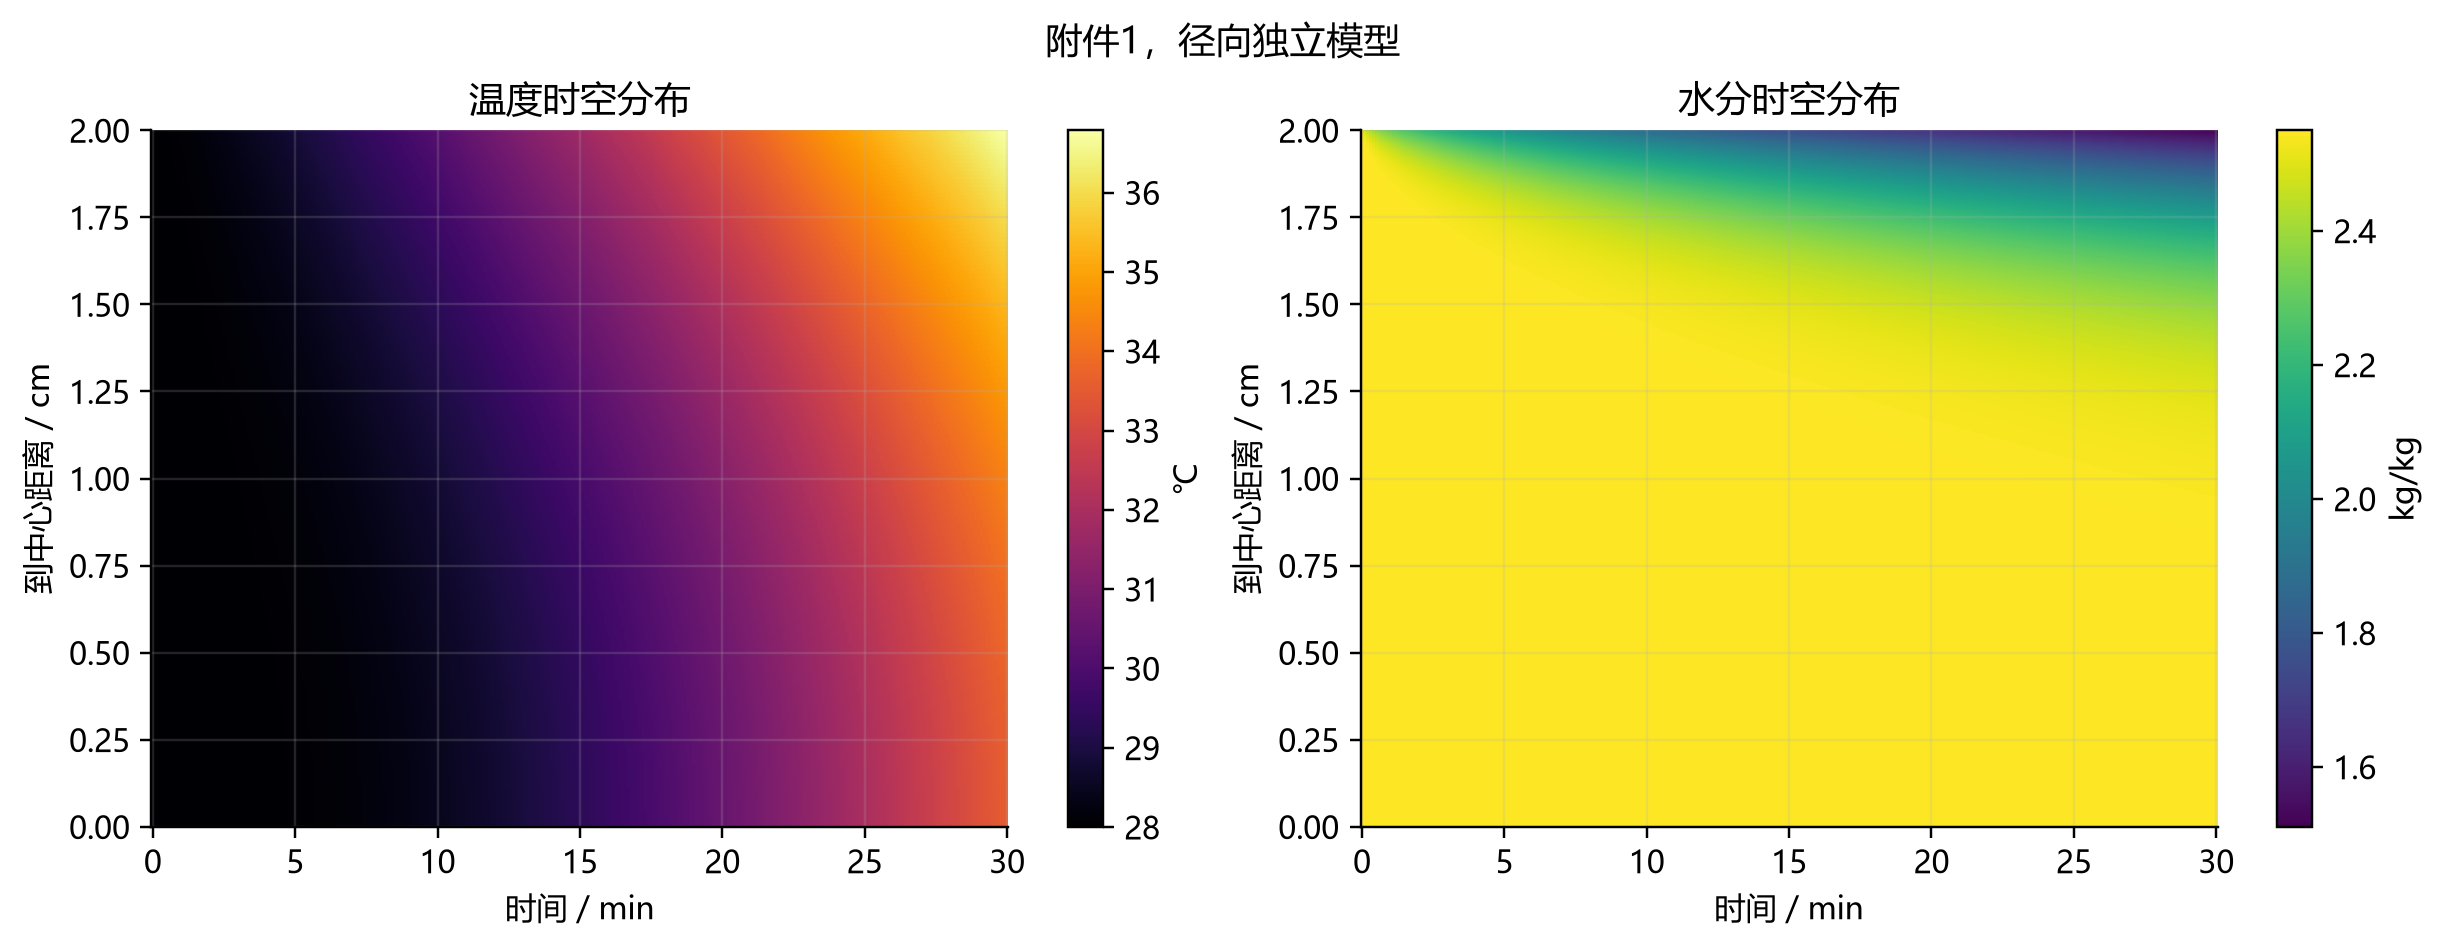
\includegraphics[width=0.85\textwidth]{fig3.png}
\caption{温度场与水分场的时空云图}
\label{fig:q1field}
\end{figure}

\begin{figure}[H]
\centering
% \includegraphics[width=0.85\textwidth]{fig_q1_center.png}
\caption{中心与表面温度、水分浓度随时间变化曲线}
\label{fig:q1center}
\end{figure}

由量级分析可知，热扩散特征时间约 \(39.5\mathrm{min}\)，水分扩散特征时间约 \(22.5\mathrm{h}\)，两者相差约两个数量级。\(1800\mathrm{s}\) 时中心温度约 \(33.6^\circ\mathrm{C}\)，表面温度约 \(36.8^\circ\mathrm{C}\)；中心含水率仍约 \(2.5500\)，表面含水率已降至约 \(1.5102\)。中心含水率在四位小数下显示为 \(2.5500\)，并不意味着数学上严格不变，而是变化量低于当前输出精度，并非数值停滞。

为进一步定量描述水分变化向内部推进的程度，定义相对失水率
\begin{equation}
\xi(r,t)=\frac{C_0-C(r,t)}{C_0},
\end{equation}
对于给定阈值 \(\eta\)，定义失水深度 \(d_\eta(t)\) 为满足 \(C(r,t)=(1-\eta)C_0\) 的径向位置到表面的距离：
\begin{equation}
d_\eta(t)=R-r_\eta(t),\qquad C(r_\eta(t),t)=(1-\eta)C_0.
\end{equation}
其中 \(r_\eta(t)\) 由相邻节点插值求根得到；若表面尚未达到该阈值，则标记为“未达到”，不人为外推。失水深度是阈值指标，不是物理界面。本文正文仅报告 \(5\%\) 失水深度，其余阈值结果放附录。计算表明 \(1800\mathrm{s}\) 内 \(5\%\) 失水深度约 \(5.69\mathrm{mm}\)，说明水分变化主要集中在距表面约 \(5\sim6\mathrm{mm}\) 的浅层。失水深度的定位误差与阈值附近的浓度梯度有关，浓度梯度越小，同一浓度误差对应更大的深度误差，报告时应同时说明其定位精度。

\subsubsection{数值验证}

图~\ref{fig:q1verify} 给出温度解析基准与数值解对比曲线，以及网格收敛误差 log-log 图。左图表明温度数值解与圆柱 Robin 边界的 Bessel--Duhamel 级数解在指定时空节点上高度一致；右图表明逐级加密网格后相邻网格差稳定下降，观测收敛阶与理论预期相符。这两项检验分别针对空间离散实现和时间积分精度，属于数值 verification，用于说明给定模型被正确、稳定地求解，不等同于真实药材实验验证。

\begin{figure}[H]
\centering
% \includegraphics[width=0.85\textwidth]{fig_q1_verify.png}
\caption{温度解析基准对比与网格收敛误差}
\label{fig:q1verify}
\end{figure}

\subsubsection{结果小结}

问题一结果呈现四个特征：第一，热扩散与水分扩散的时间尺度相差约两个数量级，\(1800\mathrm{s}\) 内温度已深入中心，而水分变化仍集中于表层；第二，\(5\%\) 失水深度约 \(5.69\mathrm{mm}\)，可定量描述水分变化向内部推进的程度；第三，初始表面瞬态使前几秒表面含水率近似按 \(\sqrt{t}\) 规律变化，是全时段误差的主要来源；第四，内部扩散与表面传质对空间分布的作用方向不同，需结合径向剖面加以区分。

\subsection{数值参数与模型假设的灵敏度分析}

题目明确给出的固定参数，如 \(h=25~\mathrm{W/(m^2\cdot K)}\)、\(h_m=8\times10^{-7}~\mathrm{m/s}\)、\(C_0=2.55~\mathrm{kg/kg}\)、\(T_0=28~^\circ\mathrm{C}\)、\(R=2~\mathrm{cm}\)、\(L=25~\mathrm{cm}\)，均视为已知条件，不纳入灵敏度分析。本文只考察题目未完全锁死、但会影响结果的三类量：水分扩散经验式的系数、常数物性假设、数值离散参数。

\subsubsection{经验式系数的敏感性}

问题一中水分扩散系数为
\begin{equation}
D(C)=A_De^{-b/C},\qquad A_D=7\times10^{-9},\quad b=0.89.
\end{equation}
该式来自题目附录，属于经验式，其系数本身带有不确定性。为考察经验式系数对结果的影响，分别对 \(A_D\) 和 \(b\) 作小幅度扰动，定义相对灵敏度
\begin{equation}
S_p^C(r,t)\approx\frac{C(r,t;p(1+\epsilon))-C(r,t;p(1-\epsilon))}{2\epsilon C_0},
\end{equation}
其中 \(p\) 取 \(A_D\) 或 \(b\)，\(\epsilon\) 取 \(2\%\)，并用 \(1\%\)、\(5\%\) 检查差分稳定性。结果表明，增大 \(A_D\) 会整体增强水分扩散能力，使表面和内部含水率同时下降；增大 \(b\) 会使 \(D\) 随 \(C\) 下降更快，药材越干越难失水，导致后期干燥速率明显降低。这说明指数系数 \(b\) 比前置系数 \(A_D\) 对后期干燥行为更敏感，若经验式存在偏差，后期含水率预测的不确定性更大。

\subsubsection{常数物性假设的敏感性}

问题一中 \(\rho\)、\(c_p\)、\(k\) 取为常数，而问题二表明它们实际随含水率变化。为说明常数假设的偏差，将问题一的常数物性替换为问题二的变物性公式，其余条件不变，重新计算 \(1800~\mathrm{s}\) 内的温度与含水率，并与原结果对比。对比指标包括中心温度、表面温度、中心含水率、表面含水率、体积平均含水率，列入表~\ref{tab:constvary_q1}。

\begin{table}[H]
\centering
\caption{常数物性与变物性在问题一条件下的对比（\(1800~\mathrm{s}\)）}
\label{tab:constvary_q1}
\begin{tabularx}{\textwidth}{|>{\centering\arraybackslash}p{3.2cm}|>{\centering\arraybackslash}X|>{\centering\arraybackslash}X|>{\centering\arraybackslash}X|}
\hline
\rowcolor{headcolor}
\textbf{指标} & \textbf{常数物性} & \textbf{变物性} & \textbf{相对偏差} \\
\hline
\rowcolor{rowcolor1}
中心温度/\(^\circ\mathrm{C}\) & 33.5753 & 待填 & 待填 \\
\hline
\rowcolor{rowcolor2}
表面温度/\(^\circ\mathrm{C}\) & 36.7856 & 待填 & 待填 \\
\hline
\rowcolor{rowcolor1}
中心含水率/(kg/kg) & 2.5500 & 待填 & 待填 \\
\hline
\rowcolor{rowcolor2}
表面含水率/(kg/kg) & 1.5102 & 待填 & 待填 \\
\hline
\rowcolor{rowcolor1}
体积平均含水率/(kg/kg) & 待填 & 待填 & 待填 \\
\hline
\end{tabularx}
\end{table}

结果表明，% 待补：填写偏差方向与量级。
这说明在预热平衡阶段，常数物性假设对温度场影响有限，但对水分场，尤其是表面含水率和体积平均含水率，可能带来不可忽略的偏差。

\subsubsection{数值离散参数的敏感性}

数值离散参数虽不影响物理模型，但直接影响结果可信度。本文考察三类数值参数：网格数 \(N\)，分别取 \(160\)、\(320\)、\(640\)、\(1280\)、\(2560\)，比较相邻网格的解；时间容差，加严 BDF 的相对与绝对容差，比较时间积分误差；Kirchhoff 通量中的 Gauss 点数，分别取 \(3\)、\(5\)、\(8\)，比较界面水分通量积分误差。网格加密时，相邻网格差稳定下降，观测收敛阶与理论预期相符；时间容差加严后，结果变化远小于空间离散误差；Gauss 点数由 \(5\) 增至 \(8\) 时，通量差远小于空间误差。这说明本文采用的空间网格、时间容差与通量积分精度足以支撑四位小数输出，数值结果对离散参数不敏感。

上述三类灵敏度分析均不改变题目给定的固定参数，只考察经验式不确定性、模型假设偏差和数值离散误差，因此不违背题目条件，同时说明结果的稳健性与适用边界。
\section{问题二的建立与求解}

\subsection{问题二的前提与建模范围}

问题二继续研究同一根圆柱形药材，但把问题一中的常数物性替换为随含水率变化的物性，并让水分扩散系数同时依赖温度和含水率，因此温度场与水分场必须联立推进，而不能像问题一那样分开求解。药材半径 \(R=0.02~\mathrm{m}\)、长度 \(L=0.25~\mathrm{m}\)，端面与侧面积之比仅 \(0.08\)，故忽略轴向梯度和端面交换，仅考虑 \(0\le r\le R\) 的一维径向问题；问题二暂不加入收缩。干基含水率定义为 \(C=m_w/m_d\)，初始状态取 \(T(r,0)=28~^\circ\mathrm{C}\)、\(C(r,0)=2.55~\mathrm{kg/kg}\)，从与问题一相同的初态重新计算，不承接问题一末态；表面换热系数 \(h=25~\mathrm{W/(m^2\cdot K)}\)、传质系数 \(h_m=8\times10^{-7}~\mathrm{m/s}\) 沿用问题一，作为模型延续假设。表~\ref{tab:q1q2} 给出两问的核心区别。

\begin{table}[H]
\centering
\caption{问题一与问题二的核心区别}
\label{tab:q1q2}
\begin{tabularx}{\textwidth}{|>{\centering\arraybackslash}p{3cm}|>{\centering\arraybackslash}X|>{\centering\arraybackslash}X|}
\hline
\rowcolor{headcolor}
\textbf{比较项} & \textbf{问题一} & \textbf{问题二} \\
\hline
\rowcolor{rowcolor1}
任务范围 & 预热平衡阶段，前 \(1800~\mathrm{s}\) & 全过程模型，前 \(3~\mathrm{h}\) \\
\hline
\rowcolor{rowcolor2}
密度 & 常数 \(820~\mathrm{kg/m^3}\) & 随含水率变化 \\
\hline
\rowcolor{rowcolor1}
比热容 & 常数 \(2600~\mathrm{J/(kg\cdot K)}\) & 随含水率变化 \\
\hline
\rowcolor{rowcolor2}
导热系数 & 常数 \(0.36~\mathrm{W/(m\cdot K)}\) & 随含水率变化 \\
\hline
\rowcolor{rowcolor1}
水分扩散系数 & 仅依赖 \(C\) & 同时依赖 \(C\) 和 \(T_K\) \\
\hline
\rowcolor{rowcolor2}
热湿关系 & 两方程可独立推进 & 两方程必须联立推进 \\
\hline
\rowcolor{rowcolor1}
起始状态 & \(28~^\circ\mathrm{C}\)，\(2.55~\mathrm{kg/kg}\) & 从同一初态重新开始 \\
\hline
\rowcolor{rowcolor2}
边界交换系数 & 附录2给出 \(h\)、\(h_m\) & 沿用前问数值，须列为假设 \\
\hline
\end{tabularx}
\end{table}

\subsection{模型建立}

\subsubsection{物性随含水率与温度变化}

问题二的物性参数直接使用题目附录3，不重新拟合系数：
\begin{align}
\rho(C) &= 650+128C,\\
c_p(C) &= 1450+2736\frac{C}{C+1},\\
k(C) &= 0.21+0.38\frac{C}{C+1},\\
B(C) &= \rho(C)c_p(C),\\
D(C,T_K) &= 2.4\times10^{-3}\exp\!\left(-\frac{0.45}{C}\right)\exp\!\left(-\frac{3850}{T_K}\right).
\end{align}
其中 \(B\) 为体积热容，单位 \(\mathrm{J/(m^3\cdot K)}\)。编程时每次根据当前 \(C\)、\(T\) 计算。

\subsubsection{温度方程}

温度场满足
\begin{equation}
B(C)\frac{\partial T}{\partial t}=\frac{1}{r}\frac{\partial}{\partial r}\left[rk(C)\frac{\partial T}{\partial r}\right].
\label{eq:q2heat}
\end{equation}
左边是单位体积的瞬时储热率，右边是附近热量流入与流出的差。热流密度为
\begin{equation}
q_r^T=-k(C)\frac{\partial T}{\partial r},
\end{equation}
向外为正。变导热系数必须留在导数里面，不能直接套用常系数的 \(k\) 乘拉普拉斯算子。本文实现仍用通量形式，让相邻圆环交换自动一致。

\subsubsection{含水率方程与双向耦合}

含水率场满足
\begin{equation}
\frac{\partial C}{\partial t}=\frac{1}{r}\frac{\partial}{\partial r}\left[rD(C,T_K)\frac{\partial C}{\partial r}\right].
\label{eq:q2moisture}
\end{equation}
含水率改变热容和导热能力，进而影响温度；温度改变扩散能力，进而影响含水率。但这种耦合来自物性更新，不能直接解释为已经包含蒸发潜热等情况的全部热湿机制。

\subsubsection{无量纲化与 Lewis 数}

为比较热扩散和水分扩散的速度，引入热扩散率
\begin{equation}
\alpha(C)=\frac{k(C)}{B(C)},
\end{equation}
以及 Lewis 数
\begin{equation}
Le=\frac{\alpha}{D}=\frac{k(C)}{B(C)D(C,T_K)}.
\label{eq:lewis}
\end{equation}
\(Le\) 表示热扩散与水分扩散的速度比。\(Le\gg1\) 意味着热量传播远快于水分迁移，因此温度先趋于均匀，水分则慢慢向外扩散。

代入初始状态可估算：
\begin{equation}
\rho_0=\rho(2.55)=650+128\times2.55=976.4~\mathrm{kg/m^3},
\end{equation}
\begin{equation}
c_{p,0}=1450+2736\times\frac{2.55}{3.55}\approx3415.2~\mathrm{J/(kg\cdot K)},
\end{equation}
\begin{equation}
B_0=\rho_0c_{p,0}\approx3.335\times10^6~\mathrm{J/(m^3\cdot K)},
\end{equation}
\begin{equation}
k_0=0.21+0.38\times\frac{2.55}{3.55}\approx0.483~\mathrm{W/(m\cdot K)},
\end{equation}
\begin{equation}
\alpha_0=\frac{k_0}{B_0}\approx1.448\times10^{-7}~\mathrm{m^2/s},
\end{equation}
\begin{equation}
D_0=2.4\times10^{-3}e^{-0.45/2.55}e^{-3850/301.15}\approx5.642\times10^{-9}~\mathrm{m^2/s},
\end{equation}
\begin{equation}
Le_0=\frac{\alpha_0}{D_0}\approx2.57\times10^1.
\end{equation}
即初始 Lewis 数约为 \(25.7\)，远大于 \(1\)。这与问题二结果中“温度先平衡、水分慢慢干”的现象一致。

进一步定义热扩散特征时间和水分扩散特征时间：
\begin{equation}
\tau_T\sim\frac{R^2}{\alpha_0},\qquad \tau_C\sim\frac{R^2}{D_0}.
\end{equation}
代入 \(R=0.02~\mathrm{m}\)：
\begin{equation}
\tau_T\approx\frac{0.02^2}{1.448\times10^{-7}}\approx2762~\mathrm{s}\approx46.0~\mathrm{min},
\end{equation}
\begin{equation}
\tau_C\approx\frac{0.02^2}{5.642\times10^{-9}}\approx7.09\times10^4~\mathrm{s}\approx19.7~\mathrm{h}.
\end{equation}
两者相差约两个数量级，说明在 \(3~\mathrm{h}\) 内温度已接近均匀，而水分仍存在明显径向梯度。

\subsubsection{边界条件与初始条件}

初始条件为
\begin{equation}
T(r,0)=28~^\circ\mathrm{C},\qquad C(r,0)=2.55~\mathrm{kg/kg}.
\end{equation}
圆心对称边界为
\begin{equation}
\frac{\partial T}{\partial r}(0,t)=0,\qquad \frac{\partial C}{\partial r}(0,t)=0.
\end{equation}
表面为 Robin 边界：
\begin{equation}
-k(C)\frac{\partial T}{\partial r}\bigg|_{r=R}=h\left[T(R,t)-T_\infty(t)\right],
\end{equation}
\begin{equation}
-D(C,T_K)\frac{\partial C}{\partial r}\bigg|_{r=R}=h_m\left[C(R,t)-C_e(t)\right].
\end{equation}
其中 \(h=25~\mathrm{W/(m^2\cdot K)}\)，\(h_m=8\times10^{-7}~\mathrm{m/s}\)，沿用问题一数值，作为模型延续假设。环境温度 \(T_\infty(t)\) 与环境水分驱动量 \(C_e(t)\) 由附件1经分段线性插值得到，不在 \(1800~\mathrm{s}\) 后人为改成恒温。

\subsection{模型求解}

\subsubsection{空间离散：圆环有限体积法}

采用有限体积法，将半径 \(0\le r\le R\) 划分为 \(N\) 个区间，节点数 \(N+1\)。节点、界面、体积和面积分别为
\begin{equation}
r_0=0,\quad r_N=R,\quad r_{i+1/2}=\frac{r_i+r_{i+1}}{2},
\end{equation}
\begin{equation}
V_i=\pi L\left(r_{i+1/2}^2-r_{i-1/2}^2\right),\qquad S_{i+1/2}=2\pi Lr_{i+1/2}.
\end{equation}
最外层和圆心都有自己的控制体，不能省掉它们的储存量。外圈体积通常更大，因此不能把每个半径点都视为同样大的一份药材。

为提升表面附近早期分辨率，采用 sinh 网格：
\begin{equation}
x_i=\frac{i}{N},\qquad r_i=R\left[1-\frac{\sinh(\beta(1-x_i))}{\sinh\beta}\right],
\end{equation}
取 \(\beta=2.5\)。网格收敛比较时固定映射和 \(\beta\)，仅改变 \(N\)。

\subsubsection{热通量}

相邻节点之间采用调和平均导热系数：
\begin{equation}
k_{i+1/2}=\frac{2k_ik_{i+1}}{k_i+k_{i+1}}.
\end{equation}
界面热流为
\begin{equation}
F_{i+1/2}^T=-S_{i+1/2}k_{i+1/2}\frac{T_{i+1}-T_i}{r_{i+1}-r_i}.
\end{equation}
所有控制面统一规定向外为正。温度更新为
\begin{equation}
\frac{\mathrm{d}T_i}{\mathrm{d}t}=\frac{F_{i-1/2}^T-F_{i+1/2}^T}{B(C_i)V_i}.
\end{equation}
圆心内侧通量为零，表面通量为
\begin{equation}
F_{N+1/2}^T=S_Rh\left[T_N-T_\infty(t)\right].
\end{equation}

\subsubsection{水分通量：非线性势差}

将扩散系数拆成温度因子和含水率因子：
\begin{equation}
A(T_K)=2.4\times10^{-3}e^{-3850/T_K},\qquad f(C)=e^{-0.45/C}.
\end{equation}
定义势函数
\begin{equation}
\Phi(C)=\int_0^Cf(z)\,\mathrm{d}z.
\end{equation}
界面水分通量为
\begin{equation}
F_{i+1/2}^C=-S_{i+1/2}A(T_{K,i+1/2})\frac{\Delta\Phi_{i+1/2}}{r_{i+1}-r_i},
\end{equation}
\begin{equation}
\Delta\Phi_{i+1/2}=\int_{C_i}^{C_{i+1}}e^{-0.45/z}\,\mathrm{d}z.
\end{equation}
用 5 点 Gauss 求积计算该积分，并与 3 点、8 点结果比较，可在保证精度的同时避免相消误差。含水率更新为
\begin{equation}
\frac{\mathrm{d}C_i}{\mathrm{d}t}=\frac{F_{i-1/2}^C-F_{i+1/2}^C}{V_i}.
\end{equation}

\subsubsection{时间推进：自适应隐式 BDF}

空间离散后，每个节点有两个未知量，原偏微分方程变成一组常微分方程
\begin{equation}
\frac{\mathrm{d}y}{\mathrm{d}t}=f(t,y),\qquad y=[T_0,C_0,T_1,C_1,\dots]^\mathsf{T}.
\end{equation}
采用 SciPy 的 BDF 自适应求解器，相对容差 \(10^{-13}\)，温度、含水率绝对容差分别 \(10^{-14}\)、\(10^{-15}\)，最大内部步长 \(5~\mathrm{s}\)。每个环境折点重新分段，每段以上一段的终值作为初值。每 \(1~\mathrm{s}\) 记录一次，但输出间隔不等于内部步长。

\subsubsection{冻结物性解析辅助解}

为验证数值实现，人为选取参考状态，把物性固定，构造一个更容易获得解析解的辅助题。温度辅助题取 \(\kappa=k^*/B^*\)、\(\mathrm{Bi}=hR/k^*\)；含水率辅助题取 \(\kappa=D^*\)、\(\mathrm{Bi}=h_mR/D^*\)。圆柱 Robin 边界的解析解为
\begin{equation}
u=g(t)+\sum_nY_nJ_0(\mu_nr/R)\int_0^t e^{-\lambda_n(t-\tau)}g'(\tau)\,\mathrm{d}\tau,
\end{equation}
其中
\begin{equation}
\lambda_n=\kappa\frac{\mu_n^2}{R^2},\qquad Y_n=\frac{2J_1(\mu_n)}{\mu_n\left[J_0^2(\mu_n)+J_1^2(\mu_n)\right]}.
\end{equation}
比较模态数加倍后的结果，先控制解析级数截断误差，再与数值解比较。真实计算仍使用变物性，不能把辅助题当作问题二答案。

\subsection{结果分析}

\subsubsection{题目指定结果}

根据上述模型和求解方法，计算得到 \(0.5\)、\(1.0\)、\(1.5\)、\(2.0\)、\(2.5\)、\(3.0~\mathrm{h}\) 时距药材中心 \(0\)、\(0.5\)、\(1\)、\(1.5\)、\(2~\mathrm{cm}\) 处的温度和含水率，分别列入表~\ref{tab:q2T} 和表~\ref{tab:q2C}。完整结果（\(10800~\mathrm{s}\) 内每隔 \(1~\mathrm{s}\)、径向 \(21\) 个输出半径）保存至 \texttt{result2.xlsx}。

\begin{table}[H]
\centering
\caption{规定时刻的温度（\(^\circ\mathrm{C}\)）}
\label{tab:q2T}
\begin{tabularx}{\textwidth}{|>{\centering\arraybackslash}p{1.8cm}|*{5}{>{\centering\arraybackslash}X|}}
\hline
时间/h & \(r=0\) & \(0.5~\mathrm{cm}\) & \(1~\mathrm{cm}\) & \(1.5~\mathrm{cm}\) & \(2~\mathrm{cm}\) \\
\hline
0.5 & 32.1892 & 32.3821 & 32.9659 & 33.9608 & 35.4130 \\
\hline
1.0 & 40.3816 & 40.5536 & 41.0605 & 41.8782 & 42.9976 \\
\hline
1.5 & 45.8468 & 45.9348 & 46.1930 & 46.6051 & 47.1400 \\
\hline
2.0 & 48.4502 & 48.4881 & 48.5984 & 48.7736 & 49.0033 \\
\hline
2.5 & 49.4670 & 49.4792 & 49.5136 & 49.5653 & 49.6609 \\
\hline
3.0 & 49.8495 & 49.8553 & 49.8746 & 49.9101 & 49.9664 \\
\hline
\end{tabularx}
\end{table}

\begin{table}[H]
\centering
\caption{规定时刻的含水率（kg/kg）}
\label{tab:q2C}
\begin{tabularx}{\textwidth}{|>{\centering\arraybackslash}p{1.8cm}|*{5}{>{\centering\arraybackslash}X|}}
\hline
时间/h & \(r=0\) & \(0.5~\mathrm{cm}\) & \(1~\mathrm{cm}\) & \(1.5~\mathrm{cm}\) & \(2~\mathrm{cm}\) \\
\hline
0.5 & 2.5499 & 2.5489 & 2.5256 & 2.3257 & 1.6486 \\
\hline
1.0 & 2.5257 & 2.4948 & 2.3578 & 2.0230 & 1.4711 \\
\hline
1.5 & 2.3861 & 2.3256 & 2.1344 & 1.8020 & 1.3476 \\
\hline
2.0 & 2.1709 & 2.1084 & 1.9236 & 1.6259 & 1.2311 \\
\hline
2.5 & 1.9566 & 1.9006 & 1.7360 & 1.4720 & 1.1166 \\
\hline
3.0 & 1.7662 & 1.7165 & 1.5702 & 1.3333 & 1.0081 \\
\hline
\end{tabularx}
\end{table}

\subsubsection{温度与含水率的时空演化}

图~\ref{fig:q2field} 给出温度场与含水率的时空云图。横轴为时间，纵轴为距中心距离，颜色表示数值大小。

\begin{figure}[H]
\centering
% \includegraphics[width=0.85\textwidth]{fig_q2_field.png}
\caption{温度与含水率的时空演化。上：温度；下：含水率。}
\label{fig:q2field}
\end{figure}

图能支持的结论：外层先升温、先失水，随后变化向内传播。末期温度图沿半径颜色接近，含水率图仍保持明显分层。整个过程中表面与圆心最大温差约 \(3.2938~^\circ\mathrm{C}\)，发生在 \(2050~\mathrm{s}\)（约 \(34.17~\mathrm{min}\)）；\(3~\mathrm{h}\) 末态温差仅 \(0.1169~^\circ\mathrm{C}\)。

\subsubsection{径向剖面与内外差异}

图~\ref{fig:q2profile} 给出六个时刻的温度剖面和含水率剖面。

\begin{figure}[H]
\centering
% \includegraphics[width=0.85\textwidth]{fig_q2_profile.png}
\caption{六个时刻的温度剖面与含水率剖面。}
\label{fig:q2profile}
\end{figure}

温度剖面后期逐渐平坦，含水率剖面仍有明显坡度。表~\ref{tab:q2diff} 给出表面与中心的温差、中心与表面的含水率差。

\begin{table}[H]
\centering
\caption{表面与中心的温差、中心与表面的含水率差}
\label{tab:q2diff}
\begin{tabular}{|c|c|c|}
\hline
时间/h & 表面$-$中心温差/\(^\circ\mathrm{C}\) & 中心$-$表面含水率/(kg/kg) \\
\hline
0.5 & 3.2238 & 0.9013 \\
\hline
1.0 & 2.6160 & 1.0546 \\
\hline
1.5 & 1.2933 & 1.0385 \\
\hline
2.0 & 0.5531 & 0.9398 \\
\hline
2.5 & 0.1939 & 0.8400 \\
\hline
3.0 & 0.1169 & 0.7581 \\
\hline
\end{tabular}
\end{table}

\subsubsection{常数物性与变物性结果对比}

为说明“物性取常数”与“物性随含水率变”两种算法的差别，本文在同一网格、同一时间容差、同一环境输入下，分别计算：

\begin{itemize}
\item 方案 A：物性取初值常数，\(\rho=\rho(2.55)\)、\(c_p=c_p(2.55)\)、\(k=k(2.55)\)，\(D\) 仍用变系数公式；
\item 方案 B：物性全程随含水率更新，即本文正式模型。
\end{itemize}

对比 \(3~\mathrm{h}\) 末态中心温度、表面温度、中心含水率、表面含水率、体积平均含水率，列入表~\ref{tab:constvary}。

\begin{table}[H]
\centering
\caption{常数物性与变物性结果对比（\(3~\mathrm{h}\) 末态）}
\label{tab:constvary}
\begin{tabularx}{\textwidth}{|>{\centering\arraybackslash}p{3.2cm}|>{\centering\arraybackslash}X|>{\centering\arraybackslash}X|>{\centering\arraybackslash}X|}
\hline
指标 & 方案 A：常数物性 & 方案 B：变物性 & 相对偏差 \\
\hline
中心温度/\(^\circ\mathrm{C}\) & 待填 & 49.8495 & 待填 \\
\hline
表面温度/\(^\circ\mathrm{C}\) & 待填 & 49.9664 & 待填 \\
\hline
中心含水率/(kg/kg) & 待填 & 1.7662 & 待填 \\
\hline
表面含水率/(kg/kg) & 待填 & 1.0081 & 待填 \\
\hline
体积平均含水率/(kg/kg) & 待填 & 1.3825 & 待填 \\
\hline
相对初始下降 & 待填 & 45.78\% & 待填 \\
\hline
\end{tabularx}
\end{table}

结果表明，若把物性取为常数，% 待补：填写偏差方向与量级。
这说明变系数建模不能偷懒：物性随含水率变化会显著改变含水率下降速度和温度分布。

\subsubsection{温度先平衡、水分慢干的机理}

由 5.2.4 节，初始 Lewis 数约为 \(25.7\)，热扩散特征时间约 \(46.0~\mathrm{min}\)，水分扩散特征时间约 \(19.7~\mathrm{h}\)，两者相差约两个数量级。图~\ref{fig:q2field} 和图~\ref{fig:q2profile} 正好反映这一点：\(3~\mathrm{h}\) 末温度径向差仅 \(0.1169~^\circ\mathrm{C}\)，而含水率中心与表面仍差 \(0.7581~\mathrm{kg/kg}\)。

这一机理也支持烘房“先预热、再恒温干燥”的两段工艺设计：

\begin{itemize}
\item 预热段：热量先传入药材，温度快速趋于均匀，为后续水分迁移提供温度条件；
\item 恒温干燥段：温度已基本均匀，水分在近似恒温条件下缓慢向外扩散，避免表面过早硬化。
\end{itemize}

若没有先预热而直接高温强风，表面会迅速失水、内部仍湿，容易形成“外干内湿”的应力开裂。Lewis 数远大于 1 从机理上说明，先预热再恒温干燥是符合传热传质规律的。

\subsection{模型验证与守恒性分析}

\subsubsection{数值验证体系}

本文采用多种独立检验：

\begin{itemize}
\item 冻结物性解析辅助解：检验圆柱 Robin 边界实现；
\item 空间网格加密：\(160\)、\(320\)、\(640\)、\(1280\)、\(2560\) 格比较；
\item 时间容差加严：检查时间积分误差；
\item BDF 与 Radau 交叉：排除单一求解器实现依赖；
\item 独立有限元二次重算：完整非线性模型对照；
\item 质量与能量守恒残差：检查离散收支装配。
\end{itemize}

图~\ref{fig:q2verify} 给出冻结物性解析对照与空间加密检查。

\begin{figure}[H]
\centering
% \includegraphics[width=0.85\textwidth]{fig_q2_verify.png}
\caption{冻结物性解析辅助题与空间加密检查。}
\label{fig:q2verify}
\end{figure}

空间 2560 与 3840 格差为 \(T:4.362\times10^{-7}~^\circ\mathrm{C}\)、\(C:1.887\times10^{-6}~\mathrm{kg/kg}\)；时间容差加严差为 \(T:4.818\times10^{-11}\)、\(C:6.546\times10^{-12}\)；BDF 与 Radau 差为 \(T:5.449\times10^{-11}\)、\(C:1.073\times10^{-11}\)。正文 60 项四位表示全部一致。独立有限元与正式结果的全时程最大差为 \(T:4.956\times10^{-7}~^\circ\mathrm{C}\)、\(C:3.409\times10^{-6}~\mathrm{kg/kg}\)。

\subsubsection{质量守恒检验}

定义有效含水率积分
\begin{equation}
I_C(t)=\sum_iV_iC_i(t),
\end{equation}
质量守恒残差为
\begin{equation}
R_C(t)=I_C(t)-I_C(0)+\int_0^tF_R^C(\tau)\,\mathrm{d}\tau,
\end{equation}
归一化残差为
\begin{equation}
\epsilon_C(t)=\frac{\left|R_C(t)\right|}{I_C(0)}.
\end{equation}
表面通量时间积分分别用 4 点和 8 点 Gauss 求积计算。图~\ref{fig:q2balance} 给出有效含水率积分平衡残差曲线。

\begin{figure}[H]
\centering
% \includegraphics[width=0.85\textwidth]{fig_q2_balance.png}
\caption{有效含水率积分收支与瞬时储热率残差。}
\label{fig:q2balance}
\end{figure}

最大相对残差约 \(7.931\times10^{-14}\)，说明数值计算总体减少与表面交换匹配。

\subsubsection{能量守恒检验}

热方程瞬时储热率残差为
\begin{equation}
R_T(t)=\sum_iV_iB(C_i)\frac{\mathrm{d}T_i}{\mathrm{d}t}+F_R^T(t),
\end{equation}
其中 \(F_R^T\) 为表面向外热流。图~\ref{fig:q2balance} 下排给出该残差曲线，最大残差约 \(8.882\times10^{-16}~\mathrm{W}\)。由于热方程采用 \(B(C)T_t\)，该检查只能说明所选热方程的离散组装收支匹配，不能改写成任意定义总内能的独立守恒验证。

\subsubsection{边界参数敏感性}

图~\ref{fig:q2sensitivity} 给出 \(h\) 与 \(h_m\) 分别变化 \(\pm10\%\) 时的末态变化。

\begin{figure}[H]
\centering
% \includegraphics[width=0.85cm]{fig_q2_sensitivity.png}
\caption{\(h\) 与 \(h_m\) 分别变化 \(\pm10\%\) 时的末态变化。}
\label{fig:q2sensitivity}
\end{figure}

\(h\) 变化 \(\pm10\%\) 时，\(3~\mathrm{h}\) 平均含水率范围为 \(1.3807\sim1.3847~\mathrm{kg/kg}\)，相对基准最大变化 \(0.16\%\)；\(h_m\) 变化 \(\pm10\%\) 时，平均含水率范围为 \(1.3280\sim1.4438~\mathrm{kg/kg}\)，相对基准最大变化 \(4.43\%\)。图中的横线是人为 \(\pm10\%\) 情景端点，不是置信区间。

\subsubsection{模型适用边界}

数值精度、参数敏感性、物理适用性是三件事。前两件已作计算；物性经验式、环境水分驱动关系和一维近似能否准确描述真实实验，仍需实测数据判断。程序未加入收缩、轴向传热、蒸发潜热等新机制，这些属于模型适用范围讨论，不能声称已经研究。

\begin{table}[H]
\centering
\caption{3小时内药材的温度}
\begin{tabularx}{\textwidth}{|>{\centering\arraybackslash}p{2.5cm}|*{5}{>{\centering\arraybackslash}X|}}
\hline
\multirow{2}{*}{时间/h} & \multicolumn{5}{c|}{到药材中心的距离/cm} \\
\cline{2-6}
 & 0 & 0.5 & 1 & 1.5 & 2 \\
\hline
0.5 &  &  &  &  &  \\
\hline
1.0 &  &  &  &  &  \\
\hline
1.5 &  &  &  &  &  \\
\hline
2.0 &  &  &  &  &  \\
\hline
2.5 &  &  &  &  &  \\
\hline
3.0 &  &  &  &  &  \\
\hline
\end{tabularx}
\end{table}

\begin{table}[H]
\centering
\caption{3小时内药材的水分浓度}
\begin{tabularx}{\textwidth}{|>{\centering\arraybackslash}p{2.5cm}|*{5}{>{\centering\arraybackslash}X|}}
\hline
\multirow{2}{*}{时间/h} & \multicolumn{5}{c|}{到药材中心的距离/cm} \\
\cline{2-6}
 & 0 & 0.5 & 1 & 1.5 & 2 \\
\hline
0.5 &  &  &  &  &  \\
\hline
1.0 &  &  &  &  &  \\
\hline
1.5 &  &  &  &  &  \\
\hline
2.0 &  &  &  &  &  \\
\hline
2.5 &  &  &  &  &  \\
\hline
3.0 &  &  &  &  &  \\
\hline
\end{tabularx}
\end{table}

\section{问题三的建立与求解}

\subsection{问题三的前提与建模范围}

问题三沿用问题二建立的固定尺寸一维径向变物性热湿耦合模型，但把任务从“给定时间求状态”改为“给定阈值求时间”：已知含水率阈值 \(C_{\mathrm{crit}}=0.15~\mathrm{kg/kg}\) 和“各处达标”的要求，求全域最大含水率首次下降至阈值以下的临界时间。药材半径 \(R=0.02~\mathrm{m}\)、长度 \(L=0.25~\mathrm{m}\)，端面与侧面积之比仅 \(0.08\)，仍忽略轴向梯度和端面交换；问题三暂不加入收缩。初始状态取 \(T(r,0)=28~^\circ\mathrm{C}\)、\(C(r,0)=2.55~\mathrm{kg/kg}\)，从与问题二相同的初态重新计算，不承接问题二末态。

与问题二相比，问题三新增两个难点：

\begin{itemize}
\item 附件 1 只覆盖 \(0\sim14400~\mathrm{s}\)（4 h），而烘干时间通常远超 4 h，需要建立 4 h 以后的长期环境假设；
\item 结束时刻未知，需要在全部计算网格上监测最大含水率，定位下降穿越，并把场误差换算为时间误差。
\end{itemize}

表~\ref{tab:q2q3} 给出问题二与问题三的核心区别。

\begin{table}[H]
\centering
\caption{问题二与问题三的核心区别}
\label{tab:q2q3}
\begin{tabularx}{\textwidth}{|>{\centering\arraybackslash}p{3cm}|>{\centering\arraybackslash}X|>{\centering\arraybackslash}X|}
\hline
\rowcolor{headcolor}
\textbf{比较项} & \textbf{问题二} & \textbf{问题三} \\
\hline
\rowcolor{rowcolor1}
任务 & 给定时间，求温度与含水率场 & 给定阈值，求全域首次达标时间 \\
\hline
\rowcolor{rowcolor2}
输出 & 温度与含水率时空分布 & 烘干时间与含水率场 \\
\hline
\rowcolor{rowcolor1}
环境范围 & 附件 1 覆盖 \(0\sim3~\mathrm{h}\) & 附件 1 覆盖 \(0\sim4~\mathrm{h}\)，之后需长期假设 \\
\hline
\rowcolor{rowcolor2}
结束条件 & 固定 \(3~\mathrm{h}\) & 全域最大含水率首次低于 \(0.15~\mathrm{kg/kg}\) \\
\hline
\rowcolor{rowcolor1}
新增难点 & 变物性耦合 & 长期环境、事件定位、时间误差 \\
\hline
\end{tabularx}
\end{table}

\subsection{模型建立}

\subsubsection{物性随含水率与温度变化}

问题三完全继承问题二的物性公式，直接使用题目附录 3，不重新拟合：
\begin{align}
\rho(C) &= 650+128C,\\
c_p(C) &= 1450+2736\frac{C}{C+1},\\
k(C) &= 0.21+0.38\frac{C}{C+1},\\
B(C) &= \rho(C)c_p(C),\\
D(C,T_K) &= 2.4\times10^{-3}\exp\!\left(-\frac{0.45}{C}\right)\exp\!\left(-\frac{3850}{T_K}\right).
\end{align}
其中 \(B\) 为体积热容，单位 \(\mathrm{J/(m^3\cdot K)}\)。编程时每次根据当前 \(C\)、\(T\) 计算，不能在初始时刻算一次后全程固定。

\subsubsection{温度方程}

温度场满足
\begin{equation}
B(C)\frac{\partial T}{\partial t}=\frac{1}{r}\frac{\partial}{\partial r}\left[rk(C)\frac{\partial T}{\partial r}\right].
\label{eq:q3heat}
\end{equation}
左边是单位体积的瞬时储热率，右边是附近热量流入与流出的差。热流密度为
\begin{equation}
q_r^T=-k(C)\frac{\partial T}{\partial r},
\end{equation}
向外为正。变导热系数必须留在导数里面，不能直接套用常系数的 \(k\) 乘拉普拉斯算子。本文实现仍用通量形式，让相邻圆环交换自动一致。

\subsubsection{含水率方程}

含水率场满足
\begin{equation}
\frac{\partial C}{\partial t}=\frac{1}{r}\frac{\partial}{\partial r}\left[rD(C,T_K)\frac{\partial C}{\partial r}\right].
\label{eq:q3moisture}
\end{equation}
含水率改变热容和导热能力，进而影响温度；温度改变扩散能力，进而影响含水率。但这种耦合来自物性更新，不能直接解释为已经包含蒸发潜热等全部热湿机制。

\subsubsection{边界条件与初始条件}

初始条件为
\begin{equation}
T(r,0)=28~^\circ\mathrm{C},\qquad C(r,0)=2.55~\mathrm{kg/kg}.
\end{equation}
圆心对称边界为
\begin{equation}
\frac{\partial T}{\partial r}(0,t)=0,\qquad \frac{\partial C}{\partial r}(0,t)=0.
\end{equation}
表面为 Robin 边界：
\begin{equation}
-k(C)\frac{\partial T}{\partial r}\bigg|_{r=R}=h\left[T(R,t)-T_\infty(t)\right],
\end{equation}
\begin{equation}
-D(C,T_K)\frac{\partial C}{\partial r}\bigg|_{r=R}=h_m\left[C(R,t)-C_e(t)\right].
\end{equation}
其中 \(h=25~\mathrm{W/(m^2\cdot K)}\)，\(h_m=8\times10^{-7}~\mathrm{m/s}\)，沿用问题二数值，作为模型延续假设。

\subsubsection{长期环境假设}

附件 1 实际覆盖 \(0\sim14400~\mathrm{s}\)（4 h）。为建立 4 h 以后的长期环境边界，先对末段数据作平台判断。定义窗口均值
\begin{equation}
\overline{g}_w=\frac{1}{W}\int_{t_s-w}^{t_s}g(t)\,\mathrm{d}t,\qquad t_s=14400~\mathrm{s},
\end{equation}
其中 \(g\) 分别取环境温度或环境水分驱动量，\(W\) 为窗口长度。基准 S60 取最后 \(60~\mathrm{min}\) 时间平均，得环境温度约 \(49.9959~^\circ\mathrm{C}\)，环境水分驱动量约 \(0.0499904~\mathrm{kg/kg}\)。正式程序从附件自动计算并保留完整精度。

0 至 4 h 使用附件 1 的分段线性环境；4 h 后使用 S60 平台代表值：
\begin{equation}
t>t_b:\quad T_\infty(t)=T_\infty^*,\qquad C_e(t)=C_e^*,
\end{equation}
其中 \(t_b=14400~\mathrm{s}\)。边界变化在 4 h 处分段处理，状态温度和含水率保持连续。附件末点为 \(50.165~^\circ\mathrm{C}\) 和 \(0.04986~\mathrm{kg/kg}\)，切到 S60 后边界温度改变 \(-0.169083~^\circ\mathrm{C}\)，环境水分量改变 \(+0.00013042~\mathrm{kg/kg}\)。这是边界定义造成的小跳变，不自动意味着程序错误。

\subsubsection{全域达标判据与临界时间}

定义全域最大含水率
\begin{equation}
C_{\max}(t)=\max_{0\le r\le R}C(r,t).
\end{equation}
最大含水率回答“最湿的位置是否已经达标”。每次事件调用在全部内部计算节点上取最大值，并记录最大值所在位置；不能只使用 Excel 的 21 个输出点。

烘干结束时间定义为
\begin{equation}
t_{\mathrm{dry}}=\inf\left\{t>0:\;C_{\max}(t)<C_{\mathrm{crit}}\right\},\qquad C_{\mathrm{crit}}=0.15.
\end{equation}
这里求严格达标集合的下确界。数值上用等于阈值的事件定位临界时间，并短时继续积分核验下降穿越。若只有接触而未进入严格达标区间，不能按完成处理。所有判断使用未舍入数据。

题目要求“各处”达标，因此真正控制条件是最大值，不能用体积平均含水率代替。平均值可能已低于 0.15，但中心仍高于 0.15。

\subsection{模型求解}

\subsubsection{空间离散：圆环有限体积法}

采用与问题二相同的有限体积法，将半径 \(0\le r\le R\) 划分为 \(N\) 个区间，节点数 \(N+1\)。节点、界面、体积和面积分别为
\begin{equation}
r_0=0,\quad r_N=R,\quad r_{i+1/2}=\frac{r_i+r_{i+1}}{2},
\end{equation}
\begin{equation}
V_i=\pi L\left(r_{i+1/2}^2-r_{i-1/2}^2\right),\qquad S_{i+1/2}=2\pi Lr_{i+1/2}.
\end{equation}
最外层和圆心都有自己的控制体。为提升表面附近早期分辨率，采用 sinh 网格：
\begin{equation}
x_i=\frac{i}{N},\qquad r_i=R\left[1-\frac{\sinh(\beta(1-x_i))}{\sinh\beta}\right],
\end{equation}
取 \(\beta=2.5\)。网格收敛比较时固定映射和 \(\beta\)，仅改变 \(N\)。

\subsubsection{热通量}

相邻节点之间采用调和平均导热系数：
\begin{equation}
k_{i+1/2}=\frac{2k_ik_{i+1}}{k_i+k_{i+1}}.
\end{equation}
界面热流为
\begin{equation}
F_{i+1/2}^T=-S_{i+1/2}k_{i+1/2}\frac{T_{i+1}-T_i}{r_{i+1}-r_i}.
\end{equation}
所有控制面统一规定向外为正。温度更新为
\begin{equation}
\frac{\mathrm{d}T_i}{\mathrm{d}t}=\frac{F_{i-1/2}^T-F_{i+1/2}^T}{B(C_i)V_i}.
\end{equation}
圆心内侧通量为零，表面通量为
\begin{equation}
F_{N+1/2}^T=S_Rh\left[T_N-T_\infty(t)\right].
\end{equation}

\subsubsection{水分通量：非线性势差}

将扩散系数拆成温度因子和含水率因子：
\begin{equation}
A(T_K)=2.4\times10^{-3}e^{-3850/T_K},\qquad f(C)=e^{-0.45/C}.
\end{equation}
定义势函数
\begin{equation}
\Phi(C)=\int_0^Cf(z)\,\mathrm{d}z.
\end{equation}
界面水分通量为
\begin{equation}
F_{i+1/2}^C=-S_{i+1/2}A(T_{K,i+1/2})\frac{\Delta\Phi_{i+1/2}}{r_{i+1}-r_i},
\end{equation}
\begin{equation}
\Delta\Phi_{i+1/2}=\int_{C_i}^{C_{i+1}}e^{-0.45/z}\,\mathrm{d}z.
\end{equation}
用 5 点 Gauss 求积计算该积分，并与 3 点、8 点结果比较。含水率更新为
\begin{equation}
\frac{\mathrm{d}C_i}{\mathrm{d}t}=\frac{F_{i-1/2}^C-F_{i+1/2}^C}{V_i}.
\end{equation}

\subsubsection{时间推进：自适应隐式 BDF}

空间离散后，每个节点有两个未知量，原偏微分方程变成一组常微分方程
\begin{equation}
\frac{\mathrm{d}y}{\mathrm{d}t}=f(t,y),\qquad y=[T_0,C_0,T_1,C_1,\dots]^\mathsf{T}.
\end{equation}
采用 SciPy 的 BDF 自适应求解器。0 至 4 h 在观测折点处分段；4 h 后基准环境恒定，可试验分钟级最大步长，但是否放宽必须由时间收敛与事件检查确认。切换初期和事件附近允许自适应缩步。

\subsubsection{事件定位}

从初始时刻开始设置下降穿越事件
\begin{equation}
g_N(t)=C_{\max,N}(t)-C_{\mathrm{crit}},
\end{equation}
direction \(=-1\)，正式事件发生后可终止主积分。对每个分段保存开始、结束状态及事件信息，找到第一个有证据支持的变号区间，再在该区间定位根。

主积分在事件处终止后，应从事件状态短时继续真实积分，并关闭终止标志以获取后验状态。日志保存首次变号区间、根时间、前后状态、各自配置及误差尺度。

\subsubsection{数值验证}

问题三的校验体系包括：

\begin{itemize}
\item V0 问题二回归：相同物理模型下前 3 h 状态在规定误差内一致；
\item V1 低含水率通量与制造解：覆盖较干表层和完整非线性实现；
\item V2 空间收敛：临界时间与事件附近场随网格加密稳定；
\item V3 时间与步长收敛：长时积分误差小于分配的时间预算；
\item V4 BDF 与 Radau 交叉一致；
\item V5 首次事件与短时后验：完整历程支持首次下降穿越；
\item V6 全域与中心检查：中心控制结论有多网格数值证据；
\item V7 有效含水率积分平衡：时间累计收支在误差内闭合；
\item V8 重启一致性：重启带来的额外差异在预算内；
\item V9 窗口与长期偏移情景：量化所研究范围内环境假设的影响。
\end{itemize}

\subsection{结果分析}

\subsubsection{题目指定结果}

根据上述模型和求解方法，计算得到每 \(6~\mathrm{h}\)、距药材中心 \(0\)、\(0.5\)、\(1\)、\(1.5\)、\(2~\mathrm{cm}\) 处的含水率，以及烘干结束时间，列入表~\ref{tab:q3C}。完整结果（每隔 \(60~\mathrm{s}\)、径向 \(21\) 个输出半径）保存至 \texttt{result3.xlsx}。

\begin{table}[H]
\centering
\caption{药材烘干过程的水分浓度}
\begin{tabularx}{\textwidth}{|>{\centering\arraybackslash}p{2.5cm}|*{5}{>{\centering\arraybackslash}X|}}
\hline
\multirow{2}{*}{时间/h} & \multicolumn{5}{c|}{到药材中心的距离/cm} \\
\cline{2-6}
 & 0 & 0.5 & 1 & 1.5 & 2 \\
\hline
6  &  &  &  &  &  \\
\hline
12 &  &  &  &  &  \\
\hline
18 &  &  &  &  &  \\
\hline
$\vdots$ &  &  &  &  &  \\
\hline
烘干结束时间 &  &  &  &  &  \\
\hline
\end{tabularx}
\end{table}


\subsubsection{全域达标过程}

图~\ref{fig:q3dry} 给出全域最大含水率、中心含水率、表面含水率、体积平均含水率随时间的曲线，并叠加 \(0.15~\mathrm{kg/kg}\) 阈值线和临界时间竖线。该图用于说明何时全部达标，以及平均值为什么不能代替停止条件。

\begin{figure}[H]
\centering
% \includegraphics[width=0.85\textwidth]{fig_q3_dry.png}
\caption{全域达标过程。最大、中心、表面、体积平均含水率随时间变化，虚线为阈值，竖线为临界时间。}
\label{fig:q3dry}
\end{figure}

从图中可以看到，中心含水率与全域最大值在误差范围内一致，临界事件附近由中心控制。表面先达标，中心最后达标，因此用体积平均含水率会低估烘干时间。

\subsubsection{时空场与较湿区域演化}

图~\ref{fig:q3field} 给出含水率时空云图，叠加 \(0.15\) 等值线和少量代表剖面，并给出后期低值局部视图。该图用于展示较湿区域如何演化。

\begin{figure}[H]
\centering
% \includegraphics[width=0.85\textwidth]{fig_q3_field.png}
\caption{含水率时空场与较湿区域演化。等值线为 \(0.15~\mathrm{kg/kg}\)，右侧为后期局部放大。}
\label{fig:q3field}
\end{figure}

定义较湿区域集合
\begin{equation}
W(t)=\{r\in[0,R]:C(r,t)>C_{\mathrm{crit}}\},
\end{equation}
湿芯半径与体积占比分别为
\begin{equation}
R_{\mathrm{wet}}(t)=\max W(t),\qquad
f_{\mathrm{wet}}(t)=\frac{2}{R^2}\int_0^R\mathbf{1}_{C(r,t)>C_{\mathrm{crit}}}\,r\,\mathrm{d}r.
\end{equation}
这些量是阈值轮廓指标，不是真实锐利相变前沿。

\subsubsection{后期干燥机制}

后期温度接近平台时，含水率降低会使经验式中的扩散因子减小，可能延长后期迁移时间。实际干燥速度还取决于径向梯度和表面驱动力，因此不能仅凭 \(D\) 下降就断言哪一种因素主导。

图~\ref{fig:q3mech} 给出 \(D\)、径向梯度、表面驱动力及平均含水率下降率在同一时间轴上的对比。该图用于解释后期是否变慢。

\begin{figure}[H]
\centering
% \includegraphics[width=0.85\textwidth]{fig_q3_mech.png}
\caption{后期干燥机制。\(D\)、径向梯度、表面驱动力与平均含水率下降率对比。}
\label{fig:q3mech}
\end{figure}

\subsubsection{结果小结}

问题三结果呈现三个特征：第一，全域最大含水率首次下降至 \(0.15~\mathrm{kg/kg}\) 的时间即烘干结束时间；第二，中心与全域最大值在误差范围内一致，事件附近由中心控制，但正式判据仍使用全域最大值；第三，后期干燥速率受扩散系数下降影响明显，接近阈值时干燥速度变慢。

\subsection{灵敏度与稳健性分析}

\subsubsection{参数灵敏度：Tornado 图}

为识别对烘干时间影响最大的工艺参数，本文分别扰动初始含水率 \(C_0\)、烘房温度水平 \(T_\infty^*\)、传质系数 \(h_m\)，从同一初态重新计算，记录烘干时间变化。扰动幅度取 \(\pm10\%\)，作为人为情景，不是测量误差或置信区间。

图~\ref{fig:q3tornado} 给出烘干时间的 tornado 图，横轴为烘干时间变化，每根横条对应一个参数，按影响大小排序。

\begin{figure}[H]
\centering
% \includegraphics[width=0.85\textwidth]{fig_q3_tornado.png}
\caption{烘干时间的参数灵敏度 Tornado 图。横轴为烘干时间变化，每根横条对应一个参数。}
\label{fig:q3tornado}
\end{figure}

结果表明，传质系数 \(h_m\) 对烘干时间影响最大，其次为烘房温度水平，初始含水率影响相对最小。这说明工艺调节应优先控制表面传质能力，其次控制烘房温度。

\subsubsection{环境情景}

环境检验分两层：S0、S30、S60、S90 比较平台代表值的取法；长期温度和水分偏移比较未来边界水平的假设。图~\ref{fig:q3env} 给出窗口组与长期偏移组分开的烘干时间或相对 S60 的变化。

\begin{figure}[H]
\centering
% \includegraphics[width=0.85\textwidth]{fig_q3_env.png}
\caption{环境情景对烘干时间的影响。窗口组与长期偏移组分开。}
\label{fig:q3env}
\end{figure}

S30、S60、S90 均值差很小，只能支持窗口选择较稳定，不能据此声称未来环境不确定性很小。长期温度偏移 \(\pm1~^\circ\mathrm{C}\)、水分偏移 \(\pm0.005~\mathrm{kg/kg}\) 作为人为情景，正式报告分别给出基准事件时间与数值误差估计、窗口对照的时间范围、长期偏移情景的时间范围。

\subsubsection{网格无关性检验}

第二问重点比较 \(T\)、\(C\) 场；第三问最终答案是时间，所以网格加密必须直接比较 \(t_{\mathrm{dry}}\)。本文分别取 \(N=320\)、\(640\)、\(1280\)，记录事件时间、控制位置、表~\ref{tab:q3C} 及事件附近剖面。图~\ref{fig:q3grid} 给出不同网格下烘干时间趋于同一值的折线。

\begin{figure}[H]
\centering
% \includegraphics[width=0.85\textwidth]{fig_q3_grid.png}
\caption{网格无关性检验。不同网格密度下烘干时间趋于同一值。}
\label{fig:q3grid}
\end{figure}

网格加密时，相邻网格的烘干时间差稳定下降，观测收敛阶与理论预期相符。正式网格由时间误差估计、表~\ref{tab:q3C} 稳定性和全域最大值检查共同决定。

\subsubsection{步长无关性检验}

固定足够细的网格和同一环境，比较候选长时容差与更严格容差，再改变最大步长。候选最大步长为 \(600\)、\(300\)、\(150~\mathrm{s}\)。图~\ref{fig:q3step} 给出不同步长下烘干时间趋于同一值的折线。

\begin{figure}[H]
\centering
% \includegraphics[width=0.85\textwidth]{fig_q3_step.png}
\caption{步长无关性检验。不同最大步长下烘干时间趋于同一值。}
\label{fig:q3step}
\end{figure}

记录实际接受步长、根时间、函数调用数。若求解器本来总在 \(150~\mathrm{s}\) 以下，三个 max\_step 结果相同并不构成独立的时间收敛证据。BDF 与 Radau 交叉一致只能说明时间积分交叉一致，不能替代网格验证。

\subsubsection{误差预算}

预先确定时间误差目标：
\begin{equation}
\hat{\epsilon}_{\mathrm{num}}=\hat{\epsilon}_{\mathrm{space}}+\hat{\epsilon}_{\mathrm{time}}+\hat{\epsilon}_{\mathrm{root}}+\hat{\epsilon}_{\mathrm{other}}.
\end{equation}
各项统一以秒记录，表示所研究数值误差来源的估计预算。可先以 \(60~\mathrm{s}\) 作为总数值误差估计的候选目标；空间估计优先控制在 \(30~\mathrm{s}\) 以内，时间加严差优先控制在 \(6~\mathrm{s}\) 以内，根定位区间优先控制在 \(0.6~\mathrm{s}\) 以内。这是实施起点，不是题目规定或理论保证。

\subsubsection{模型适用边界}

数值精度、参数敏感性、物理适用性是三件事。前两件已作计算；物性经验式、环境水分驱动关系和一维近似能否准确描述真实实验，仍需实测数据判断。程序未加入收缩、轴向传热、蒸发潜热等新机制，这些属于模型适用范围讨论，不能声称已经研究。尺寸收缩按题目留给问题四；本问结果应称为固定尺寸有效模型下的预测。


\section{问题四的建立与求解}

\subsection{问题四的前提与建模范围}

问题四在问题三的基础上再增加一个变化：药材在烘干过程中半径随时间减小，表面位置不再是固定的 \(R=0.02~\mathrm{m}\)，计算区域本身在缩短。同时，物性从问题三的附录 3 换成题目附录 4 给出的另一套经验公式。因此，问题四不能沿用问题三的结果，必须从初始时刻重新计算。

表~\ref{tab:q3q4} 给出问题三与问题四的核心区别。

\begin{table}[H]
\centering
\caption{问题三与问题四的核心区别}
\label{tab:q3q4}
\begin{tabularx}{\textwidth}{|>{\centering\arraybackslash}p{3cm}|>{\centering\arraybackslash}X|>{\centering\arraybackslash}X|}
\hline
\rowcolor{headcolor}
\textbf{比较项} & \textbf{问题三} & \textbf{问题四} \\
\hline
\rowcolor{rowcolor1}
半径 & 固定 \(R=0.02~\mathrm{m}\) & 由附件 2 实测半径给定，随时间减小 \\
\hline
\rowcolor{rowcolor2}
物性 & 附录 3 & 附录 4 \\
\hline
\rowcolor{rowcolor1}
计算区域 & 固定 & 移动边界，随半径缩短 \\
\hline
\rowcolor{rowcolor2}
输出位置 & 固定径向距离 & 固定物理位置，域外留空；另列表面位置 \\
\hline
\rowcolor{rowcolor1}
核心任务 & 全域首次达标时间 & 移动区域内的首次达标时间 \\
\hline
\end{tabularx}
\end{table}

问题四可复用问题三的环形有限体积、非线性水分通量、隐式时间推进和事件框架，但几何、四个物性函数、动态校验和输出位置都需要更新。问题四从初始时刻重新计算，不能接着问题三的末态继续。

\subsubsection{必须写进论文的假设}

\begin{enumerate}
\item 药材视为轴对称长圆柱，初始长度 \(0.25~\mathrm{m}\)、半径 \(0.02~\mathrm{m}\)。只计算径向传递，忽略轴向梯度和端面交换；长度保持不变。附件 2 只给半径，不能据此推断长度也同比缩短。
\item 横截面均匀同比径向收缩，同一相对半径对应同一材料层。这个假设使网格可以跟随材料运动，但它不是附件 2 直接测出的内部变形规律。
\item 半径由观测数据预先给定，温湿场随之演化。这是单向耦合：半径影响传递，模型不另外根据含水率预测半径。
\item 沿用前问的有效热湿方程和表面对流闭合。未显式描述潜热、变形功、孔隙气流及完整组分焓输运；这些简化限制物理解释的范围。
\item 附录 4 密度用于题给热物性，不额外作为干物质密度或收缩定律。
\end{enumerate}

\subsection{模型建立}

\subsubsection{输入数据与单位统一}

输入数据和单位统一列入表~\ref{tab:q4input}。

\begin{table}[H]
\centering
\caption{问题四输入数据与单位}
\label{tab:q4input}
\begin{tabularx}{\textwidth}{|>{\centering\arraybackslash}p{3.2cm}|>{\centering\arraybackslash}X|>{\centering\arraybackslash}X|}
\hline
\rowcolor{headcolor}
\textbf{输入} & \textbf{取值或处理} & \textbf{来源及性质} \\
\hline
\rowcolor{rowcolor1}
初始状态 & \(T(\xi,0)=28~^\circ\mathrm{C}\)，\(C(\xi,0)=2.55~\mathrm{kg/kg}\) & 题面 \\
\hline
\rowcolor{rowcolor2}
初始几何 & \(R_0=0.02~\mathrm{m}\)，\(L=0.25~\mathrm{m}\) & 题面；长度固定是简化 \\
\hline
\rowcolor{rowcolor1}
交换系数 & \(h=25~\mathrm{W/(m^2\cdot K)}\)，\(h_m=8\times10^{-7}~\mathrm{m/s}\) & 附录 2，后续问沿用的闭合选择 \\
\hline
\rowcolor{rowcolor2}
环境记录 & 附件 1，\(0\sim14400~\mathrm{s}\) & 区间内分段线性插值 \\
\hline
\rowcolor{rowcolor1}
半径记录 & 附件 2 & 区间内保持单调的 PCHIP 插值 \\
\hline
\end{tabularx}
\end{table}

内部一律使用秒、米、摄氏温度状态和干基含水率；扩散系数函数内部先转成开尔文。图表可显示小时和厘米，但必须在接口处明确换算。

\subsubsection{半径输入与插值}

将附件 2 的厘米转换成米，先检查时间严格递增、半径有限且为正、记录单调不增，再使用保持单调的 PCHIP 插值。它通过所有观测点且一阶导连续，二阶导不必连续，不要笼统称为“完全光滑”。\(72~\mathrm{h}\) 之后关闭插值器默认外推，显式处理：
\begin{equation}
R(t)=R_{\mathrm{PCHIP}}(t)\quad(0\le t\le 259200~\mathrm{s}),
\end{equation}
\begin{equation}
R(t)=0.01198~\mathrm{m}\quad(t>259200~\mathrm{s}).
\end{equation}
对照方案用相同数据的分段线性插值。需要验证全部 145 个原始节点重现、区间内正性和单调性、平台连接连续。

图~\ref{fig:q4radius} 给出附件 2 半径观测和两种插值，局部图放大早期快速变化和末段。

\begin{figure}[H]
\centering
% \includegraphics[width=0.95\textwidth]{fig_q4_radius.png}
\caption{附件 2 半径观测与两种插值。左：全程；右：早期与末段局部放大。线条只连接观测区间，未绘制未经验证的未来半径。}
\label{fig:q4radius}
\end{figure}

读图结论限于输入：半径由 \(2.000~\mathrm{cm}\) 减至 \(1.198~\mathrm{cm}\)，\(6~\mathrm{h}\) 为 \(1.374~\mathrm{cm}\)，\(12~\mathrm{h}\) 为 \(1.248~\mathrm{cm}\)，\(24~\mathrm{h}\) 为 \(1.204~\mathrm{cm}\)。67 至 \(72~\mathrm{h}\) 的记录相同，只能支持采用平台延拓作为基线，不能证明此后半径精确不变。

\subsubsection{附录 4 物性}

四个经验式必须一起切换到附录 4。下面的 \(C\) 为 \(\mathrm{kg/kg}\)，\(T_K\) 为 K；计算时用当前节点状态更新物性：
\begin{align}
\rho(C) &= 760+90C,\\
c_p(C) &= 1850+2150\frac{C}{C+1},\\
k(C) &= 0.12+0.20\frac{C}{C+1},\\
D(C,T_K) &= 4.2\times10^{-4}\exp\!\left(-\frac{0.30}{C}\right)\exp\!\left(-\frac{3850}{T_K}\right),\\
B(C) &= \rho(C)c_p(C).
\end{align}
\(\rho\) 的单位为 \(\mathrm{kg/m^3}\)，\(c_p\) 为 \(\mathrm{J/(kg\cdot K)}\)，\(k\) 为 \(\mathrm{W/(m\cdot K)}\)，\(D\) 为 \(\mathrm{m^2/s}\)，\(B\) 为 \(\mathrm{J/(m^3\cdot K)}\)。通俗地说，\(B\) 决定升温需要多少热，\(k\) 决定热向内传得多快，\(D\) 决定水分在内部迁移得多快。

在相同温度和含水率下，附录 4 与附录 3 的扩散系数之比为
\begin{equation}
\frac{D_4}{D_3}=0.175\exp\!\left(\frac{0.15}{C}\right).
\label{eq:ratioD}
\end{equation}
当 \(C=0.15\) 时此比值约为 0.476，当 \(C=0.05\) 时约为 3.515，两者在约 \(C=0.0861\) 处相等。这说明附录 4 并非在所有含水率下都更慢；直接把两问时间差归因于收缩会混入物性变化。

正式计算要求 \(C>0\)、\(T_K>0\)，并检查全部物性有限且为正。负含水率通常说明误差控制或通量实现有问题，不可静默裁剪后宣布通过。

\subsubsection{归一化材料坐标}

用当前半径作尺子，将真实半径 \(r\) 变成相对位置 \(\xi\)：
\begin{equation}
\xi=\frac{r}{R(t)},\qquad r=R(t)\xi,\qquad 0\le\xi\le1.
\label{eq:q4xi}
\end{equation}
中心始终是 \(\xi=0\)，表面始终是 \(\xi=1\)。若同一层材料始终处在总半径的四分之一处，它的编号就是 \(\xi=0.25\)；药材变细时，编号不变，真实位置变小。

图~\ref{fig:q4material} 给出固定材料层与固定物理位置的区别。三行分别对应附件 2 的 \(0\)、\(6\)、\(72~\mathrm{h}\)；同色点表示相同材料坐标，虚线表示固定 \(0.5~\mathrm{cm}\) 位置。

\begin{figure}[H]
\centering
% \includegraphics[width=0.95\textwidth]{fig_q4_material.png}
\caption{固定材料层与固定物理位置的区别。同色点表示相同材料坐标，虚线表示固定 \(0.5~\mathrm{cm}\) 位置。}
\label{fig:q4material}
\end{figure}

当网格一直固定在同一组 \(\xi_i\) 上，且材料按假设同比分布时，每次用 \(r_i=R(t)\xi_i\) 更新物理位置，同时保留 \(T_i,C_i\) 的状态定义，正是材料坐标方法。选用固定 \(\xi\) 网格后，不需要随半径减小删除外层节点，也不需要为几何变化反复插值状态。固定 \(0.5~\mathrm{cm}\) 是输出位置，随材料移动的 \(\xi=0.5\) 是内部编号，两者不同。

\subsubsection{空间导数与圆柱扩散算子}

在某个固定时刻，\(R(t)\) 对空间变量是常数。链式法则给出
\begin{equation}
\frac{\partial r}{\partial\xi}=R(t),\qquad \frac{\partial}{\partial r}=\frac{1}{R(t)}\frac{\partial}{\partial\xi},
\end{equation}
\begin{equation}
T_r=\frac{T_\xi}{R(t)},\qquad C_r=\frac{C_\xi}{R(t)}.
\end{equation}
这表示同样的相对位置差，收缩后对应更短的真实距离，因此真实空间梯度会更陡。以水分方程为例，圆柱径向扩散算子逐项变化如下：
\begin{equation}
L_c=\frac{1}{r}\frac{\partial}{\partial r}\left(rD\frac{\partial C}{\partial r}\right),
\end{equation}
\begin{equation}
rD C_r=(R\xi)D\frac{C_\xi}{R}=\xi D C_\xi,
\end{equation}
\begin{equation}
\frac{\partial}{\partial r}\left(rD C_r\right)=\frac{1}{R}\frac{\partial}{\partial\xi}\left(\xi D C_\xi\right),
\end{equation}
\begin{equation}
L_c=\frac{1}{R(t)^2}\frac{1}{\xi}\frac{\partial}{\partial\xi}\left(\xi D C_\xi\right).
\label{eq:q4operator}
\end{equation}
热扩散把 \(D,C\) 分别换成 \(k,T\)，推导完全相同。\(1/R^2\) 的两个来源是外面的 \(1/r\) 和空间求导的 \(1/R\)，不能因为中间的 \(R\) 抵消就把最终几何尺度漏掉。

中心是坐标表达的特殊点，不是物理奇点。对光滑标量 \(u\) 和正系数 \(a\)，有
\begin{equation}
\lim_{\xi\to0}\frac{1}{\xi}\frac{\partial}{\partial\xi}\left(\xi a\frac{\partial u}{\partial\xi}\right)=2a\frac{\partial^2u}{\partial\xi^2}\bigg|_{\xi=0}.
\end{equation}
实现中无需直接计算 \(1/0\)。第 5.3.1 节用具有有限体积的实心中心控制体，中心内侧面积为零，因此中心内侧通量自动为零。

\subsubsection{时间导数与材料运动}

用波浪号暂时区分同一个场的两种坐标表示：
\begin{equation}
\widetilde{C}(\xi,t)=C(R(t)\xi,t),
\end{equation}
\begin{equation}
\frac{\partial\widetilde{C}}{\partial t}\bigg|_\xi=\frac{\partial C}{\partial t}\bigg|_r+\dot{R}\xi\frac{\partial C}{\partial r},
\end{equation}
\begin{equation}
\frac{\partial C}{\partial t}\bigg|_r=\widetilde{C}_t-\frac{\dot{R}}{R}\xi\widetilde{C}_\xi.
\end{equation}
固定 \(r\) 观察，相当于把测量仪放在房间里的一个位置；固定 \(\xi\) 观察，相当于把测量仪贴在一层材料上。材料在移动，两种时间变化率自然不同。

均匀同比收缩对应的径向材料速度和材料导数为
\begin{equation}
v_r(r,t)=\frac{\dot{R}(t)}{R(t)}r=\dot{R}(t)\xi,
\end{equation}
\begin{equation}
\frac{DC}{Dt}=\frac{\partial C}{\partial t}\bigg|_r+v_rC_r=\widetilde{C}_t.
\end{equation}
因此，我们先选择含材料导数的有效物理方程，再变换到 \(\xi\)，此时移动项被材料运动包含。只有坐标变换，并不能把一个静止介质方程自动变成收缩介质方程。

\subsubsection{连续热湿模型}

主模型采用材料局部储热和有效水分扩散：
\begin{equation}
B(C)\frac{DT}{Dt}=\frac{1}{r}\frac{\partial}{\partial r}\left(rk\frac{\partial T}{\partial r}\right),
\end{equation}
\begin{equation}
\frac{DC}{Dt}=\frac{1}{r}\frac{\partial}{\partial r}\left(rD\frac{\partial C}{\partial r}\right).
\end{equation}
代入材料坐标变换，在固定区间上得到
\begin{equation}
B(C)T_t=\frac{1}{R(t)^2\xi}\frac{\partial}{\partial\xi}\left[\xi k(C)T_\xi\right],
\label{eq:q4heat}
\end{equation}
\begin{equation}
C_t=\frac{1}{R(t)^2\xi}\frac{\partial}{\partial\xi}\left[\xi D(C,T_K)C_\xi\right].
\label{eq:q4moisture}
\end{equation}
热方程的 \(B(C)T_t\) 表示当前热容量乘升温速率。不能擅自改成 \((BT)_t\)，因为后者多出 \(TB_CC_t\)，已经换了储热模型。

中心取对称条件，初始状态均匀：
\begin{equation}
T_\xi(0,t)=C_\xi(0,t)=0,\qquad T(\xi,0)=28,\qquad C(\xi,0)=2.55.
\end{equation}
表面用 \(T_s=T(1,t)\)、\(C_s=C(1,t)\)，统一将向外通量记为正。物理坐标与材料坐标下的热边界分别为
\begin{equation}
-\frac{k(C_s)}{R(t)}T_\xi(1,t)=h\left[T_s-T_\infty(t)\right],
\end{equation}
水分边界同样带上梯度尺度，扩散函数必须使用绝对温度：
\begin{equation}
-\frac{D(C_s,T_{K,s})}{R(t)}C_\xi(1,t)=h_m\left[C_s-C_e(t)\right].
\end{equation}
热风比药材热时，热通量为负，代表热从外部进入；材料比环境湿时，水分通量为正，代表向外失水。不要对通量取绝对值，否则会破坏边界方向。

\subsection{模型求解}

\subsubsection{固定材料网格与中心控制体}

取 \(N\) 个均匀径向区间，共 \(N+1\) 个节点，中心和表面都是真实未知量：
\begin{equation}
\xi_i=i/N,\quad i=0,1,\dots,N,
\end{equation}
\begin{equation}
\xi_{i+1/2}=(\xi_i+\xi_{i+1})/2,\qquad \xi_{-1/2}=0,\qquad \xi_{N+1/2}=1.
\end{equation}
节点之间的中心是控制面。每个控制体围绕一个节点；第一块是实心圆柱核心，中间是环壳，最后一块接到真实表面。体积和面积使用同一个半径函数：
\begin{equation}
r_i(t)=R(t)\xi_i,\qquad S_{i+1/2}(t)=2\pi LR(t)\xi_{i+1/2},
\end{equation}
\begin{equation}
V_i(t)=\pi LR(t)^2\left(\xi_{i+1/2}^2-\xi_{i-1/2}^2\right),
\end{equation}
\begin{equation}
V_0(t)=\pi LR(t)^2\xi_{1/2}^2,\qquad S_{-1/2}=0.
\end{equation}
第一个节点 \(C_0\) 代表中心小控制体的含水率，网格加密后趋近连续模型的中心值。中心内侧没有通量，但外侧仍可向下一层传水，不能把整个中心控制体冻结。

每次计算都能做的几何自检为
\begin{equation}
\sum_{i=0}^NV_i(t)=\pi LR(t)^2,\qquad S_{N+1/2}=2\pi LR(t),
\end{equation}
\begin{equation}
\dot{V}_i(t)=2\frac{\dot{R}(t)}{R(t)}V_i(t).
\end{equation}
第一式检查控制体是否覆盖完整圆柱；第二式检查表面面积；第三式为后面的移动平衡提供依据。

\subsubsection{内部通量与非线性水分重构}

定义正方向向外，每个内部界面只计算一次通量，左右相邻控制体使用同一个数值、相反符号。热通量使用正的调和平均系数：
\begin{equation}
k_{i+1/2}=\frac{2k_ik_{i+1}}{k_i+k_{i+1}},
\end{equation}
\begin{equation}
F_{i+1/2}^T=-S_{i+1/2}k_{i+1/2}\frac{T_{i+1}-T_i}{r_{i+1}-r_i}
=-2\pi L\xi_{i+1/2}k_{i+1/2}\frac{T_{i+1}-T_i}{\xi_{i+1}-\xi_i}.
\end{equation}
面积正比于 \(R\)，节点间距也正比于 \(R\)，所以内部通量里的显式半径抵消。储量的体积仍正比于 \(R^2\)，最后的状态变化率仍包含几何影响。

低含水率时 \(D\) 随 \(C\) 急剧变化。把一条边上所有位置都用同一个端点的 \(D\) 代替，可能误判薄的干燥层阻力。将扩散系数拆分为
\begin{equation}
D(C,T_K)=A(T_K)f(C),\qquad A(T_K)=4.2\times10^{-4}e^{-3850/T_K},\qquad f(C)=e^{-0.30/C}.
\end{equation}
定义势函数
\begin{equation}
\Phi(C)=\int_0^Cf(z)\,\mathrm{d}z,
\end{equation}
则
\begin{equation}
\Delta\Phi=\Phi(C_R)-\Phi(C_L)=(C_R-C_L)\int_0^1e^{-0.30/[C_L+s(C_R-C_L)]}\,\mathrm{d}s.
\end{equation}
界面水分通量为
\begin{equation}
F_{i+1/2}^C=-2\pi L\xi_{i+1/2}A(T_{K,i+1/2})\frac{\Delta\Phi}{\xi_{i+1}-\xi_i},
\end{equation}
\begin{equation}
T_{K,i+1/2}=\frac{T_i+T_{i+1}}{2}+273.15.
\end{equation}
这是对含水率非线性的积分处理，界面温度仍是近似，不是整个非线性问题的精确解。用 Gauss 积分计算区间积分，并比较 3、5、8 点结果；当 \(C_L=C_R\) 时直接令势差为零，避免相减误差。反转左右节点后，势差和通量都应反号。

\subsubsection{有限体积状态方程}

中心内侧通量为零，表面通量由物理边界直接给出：
\begin{equation}
F_{-1/2}^T=F_{-1/2}^C=0,
\end{equation}
\begin{equation}
F_{N+1/2}^T=2\pi LR(t)h\left[T_N-T_\infty(t)\right],
\end{equation}
\begin{equation}
F_{N+1/2}^C=2\pi LR(t)h_m\left[C_N-C_e(t)\right].
\end{equation}
对每个控制体使用“输入减输出”，得到联立常微分方程：
\begin{equation}
\frac{\mathrm{d}T_i}{\mathrm{d}t}=\frac{F_{i-1/2}^T-F_{i+1/2}^T}{B(C_i)V_i(t)},
\end{equation}
\begin{equation}
\frac{\mathrm{d}C_i}{\mathrm{d}t}=\frac{F_{i-1/2}^C-F_{i+1/2}^C}{V_i(t)}.
\end{equation}
两式中的 \(V_i(t)\) 已经包含 \(R^2\)。若使用上述真实面积通量和真实体积，就不能再把右侧乘一次 \(R^{-2}\)。同理，表面面积里的 \(R\) 不能遗漏。

\subsubsection{时间推进与事件定位}

把 \(N+1\) 个温度与 \(N+1\) 个含水率组成状态向量，采用同一固定顺序存储。BDF 在每一步根据误差估计自动选步，适合预热较快、后期失水较慢的联立系统。每次右侧计算依次取得半径与环境，更新物性、几何和界面通量，最后形成温度与水分变化率。

温度与含水率量纲不同，使用分量绝对容差。可从 \(\mathrm{rtol}=10^{-6}\)、温度 \(\mathrm{atol}=10^{-7}~^\circ\mathrm{C}\)、含水率 \(\mathrm{atol}=10^{-9}~\mathrm{kg/kg}\) 起试；这些只是候选值。后续收紧到原来的十分之一，比较事件和关键剖面，再决定正式配置。使用相邻层耦合产生的稀疏雅可比结构加速，但不能错误删掉温湿交叉依赖。

先在全域定义最大含水率，而不是提前认定中心一定最慢：
\begin{equation}
C_{\max}(t)=\max_{0\le\xi\le1}C(\xi,t),\qquad g(t)=C_{\max}(t)-0.15,
\end{equation}
\begin{equation}
t_{\mathrm{crit}}=\inf\{t>0:C_{\max}(t)<0.15\}.
\end{equation}
若场连续并发生向下穿越，这个下确界处通常满足等号。因而数值上定位 \(g(t)=0\)，将它作为临界烘干时长，同时给出根后实际积分点的严格达标检查。不能声称等号点已经严格小于阈值。

图~\ref{fig:q4event} 给出临界事件与收缩效应的对照。主图画 Q4 full 与 Q4 control 的全域最大含水率，加入 0.15 水平线；另设临界区局部图，标出根、括区与根后检查点。

\begin{figure}[H]
\centering
% \includegraphics[width=0.95\textwidth]{fig_q4_event.png}
\caption{临界事件与收缩效应。主图：Q4 full 与 Q4 control 的全域最大含水率；局部图：临界区放大。}
\label{fig:q4event}
\end{figure}

\subsection{结果分析}

\subsubsection{题目指定结果}

根据上述模型和求解方法，计算得到每 \(6~\mathrm{h}\)、距药材中心 \(0\)、\(0.5\)、\(1\)、\(1.5\)、\(2~\mathrm{cm}\) 处以及药材表面的含水率，并给出烘干结束时间，列入表~\ref{tab:q4C}。完整结果（每隔 \(60~\mathrm{s}\)、固定物理位置每隔 \(0.1~\mathrm{cm}\)）保存至 \texttt{result4.xlsx}。

\begin{table}[H]
\centering
\caption{药材烘干过程的水分浓度}
\begin{tabularx}{\textwidth}{|>{\centering\arraybackslash}p{2.5cm}|*{6}{>{\centering\arraybackslash}X|}}
\hline
\multirow{2}{*}{时间/h} & \multicolumn{6}{c|}{到药材中心的距离/cm} \\
\cline{2-7}
 & 0 & 0.5 & 1 & 1.5 & 2 & 药材表面 \\
\hline
6  &  &  &  &  &  &  \\
\hline
12 &  &  &  &  &  &  \\
\hline
18 &  &  &  &  &  &  \\
\hline
$\vdots$ &  &  &  &  &  &  \\
\hline
烘干结束时间 &  &  &  &  &  &  \\
\hline
\end{tabularx}
\end{table}

\(6~\mathrm{h}\) 时实测半径为 \(1.374~\mathrm{cm}\)，所以 1.2 和 \(1.3~\mathrm{cm}\) 仍在内部，应写入该行。\(72~\mathrm{h}\) 时半径为 \(1.198~\mathrm{cm}\)，1.2 和 \(1.3~\mathrm{cm}\) 已在外部，这些格应留空。空白表示“该位置已不属于药材”，不是“含水率为零”或“计算失败”。最后一列保持“药材表面”，每行取 \(C(1,t_k)\)，其真实位置为 \(R(t_k)\)。

\subsubsection{半径收缩与物理域、材料域含水率}

图~\ref{fig:q4field} 给出物理域含水率和材料域含水率两幅时空图。F3 中 \(r>R(t)\) 的区域必须遮罩留白，不能填零、复制边界或让插值外推。F4 的每一行相对位置均有意义，横向比较的是同一材料层。

\begin{figure}[H]
\centering
% \includegraphics[width=0.95\textwidth]{fig_q4_field.png}
\caption{物理域含水率（上）与材料域含水率（下）。上图中 \(r>R(t)\) 区域留白；两图共用时间轴和色标。}
\label{fig:q4field}
\end{figure}

两图使用同一份场数据、相同时间范围和色标范围。若增加 \(0.02\sim0.20~\mathrm{kg/kg}\) 的后期局部放大，清楚标注它使用局部色标；主图仍保留 0 至 2.55 的完整信息。阈值等值线只在场中确实存在 0.15 交界时绘制。

\subsubsection{收缩效应}

同物性对照才回答收缩的影响。Q4 control 使用附录 4 物性、固定 \(2~\mathrm{cm}\) 半径；Q4 full 使用附录 4 物性、附件 2 实测半径。两者环境、初值、边界及数值精度一致，收缩时间差为
\begin{equation}
\Delta t_{\mathrm{shrink}}=t_{\mathrm{crit,full}}-t_{\mathrm{crit,control}}.
\end{equation}
这个差值表示附录 4 及既定环境下的模型几何效应，不能称为实验因果效应。若还要分解物性与几何的交互作用，可补做“附录 3 加收缩”的第四个组合。

最终半径对应约 2.787 的内部扩散尺度倍率、约 1.669 的侧面积体积比倍率。它们解释几何机制，不等于实际失水速率也乘相同倍数。

\subsubsection{结果小结}

问题四结果呈现三个特征：第一，全域最大含水率首次下降至 \(0.15~\mathrm{kg/kg}\) 的时间即移动区域内的烘干结束时间；第二，半径收缩缩短了水分迁移路径，同物性对照下临界时间发生改变；第三，输出表在固定物理位置处必须随当前半径判定是否在域内，域外留空，不能填零或复制边界值。

\subsection{灵敏度与稳健性分析}

\subsubsection{半径输入选择}

半径幅度敏感性用保持初始半径的变换：
\begin{equation}
R_\lambda(t)=R_0-\lambda\left[R_0-R_{\mathrm{base}}(t)\right],
\end{equation}
例如 \(\lambda=0.98,1,1.02\) 仅作为扰动情景，先检查正性与单调性，不称为仪器误差范围。若事件晚于 \(72~\mathrm{h}\)，再对 \(72~\mathrm{h}\) 后的平台取值或小幅继续收缩做连续连接的独立情景，并说明新假设。

图~\ref{fig:q4radsens} 给出不同半径插值与幅度扰动下的临界时间范围。

\begin{figure}[H]
\centering
% \includegraphics[width=0.85\textwidth]{fig_q4_radsens.png}
\caption{半径插值与幅度扰动对临界时间的影响。PCHIP 与分段线性对照，\(\lambda=0.98,1,1.02\) 为人为情景。}
\label{fig:q4radsens}
\end{figure}

\subsubsection{长期环境比较}

长期环境比较末值、末 30/60/90 min 时间均值；必要时增加温度 \(\pm1~^\circ\mathrm{C}\)、环境含水率 \(\pm0.005\) 的人工情景。改变环境仍沿用实测半径，属于“半径输入固定条件下”的敏感性，不是新的真实环境收缩预测。输出各情景临界时间范围，不能把它标成 \(95\%\) 置信区间。

\subsubsection{网格无关性检验}

空间候选网格取 \(N=320,640,1280\)；必要时继续加密。以临界时间为主指标，同时比较中心、表面、表~\ref{tab:q4C} 各位置和临界剖面。不能只看曲线肉眼重合。正式配置原则上需有更细配置支撑。

图~\ref{fig:q4grid} 给出不同网格下临界时间趋于同一值的折线。

\begin{figure}[H]
\centering
% \includegraphics[width=0.85\textwidth]{fig_q4_grid.png}
\caption{网格无关性检验。不同网格密度下临界时间趋于同一值。}
\label{fig:q4grid}
\end{figure}

\subsubsection{步长无关性检验}

固定足够细网格后比较容差、最大步长，再做 BDF 与 Radau 对照；只改变一个因素，保留各自完整配置。候选最大步长为 \(600\)、\(300\)、\(150~\mathrm{s}\)。图~\ref{fig:q4step} 给出不同步长下临界时间趋于同一值的折线。

\begin{figure}[H]
\centering
% \includegraphics[width=0.85\textwidth]{fig_q4_step.png}
\caption{步长无关性检验。不同最大步长下临界时间趋于同一值。}
\label{fig:q4step}
\end{figure}

\subsubsection{数值验证体系}

问题四的验证层次包括：

\begin{itemize}
\item V1 输入与物性：节点重现、单位换算、低含水率扫描数据处理和经验式实现；
\item V2 几何：多时刻检验总体积、表面面积、节点对应材料层和真实几何一致；
\item V3 固定半径退化：同附录 4、同网格比较物理坐标与材料坐标变换与几何因子一致；
\item V4 均匀状态保持：半径变化、边界零通量，初始常数是否误把体积缩小算成状态变化；
\item V5 动态制造解：解析移动半径、非均匀温湿场、已知源项动态几何和非线性算子正确性；
\item V6 移动平衡：独立积分并细化积分采样，表面交换与有效积分量一致；
\item V7 数值收敛：网格、容差、步长、通量积分、求解器对照结果是否受数值配置影响；
\item V8 事件与导出：首次穿越、根后达标、域外掩膜题目结论和交付数据正确。
\end{itemize}

图~\ref{fig:q4verify} 给出数值验证面板。F6 拆成小图：固定半径退化、动态制造解、达标时间收敛、移动平衡残差。

\begin{figure}[H]
\centering
% \includegraphics[width=0.95\textwidth]{fig_q4_verify.png}
\caption{数值验证面板。(a) 固定半径退化；(b) 动态制造解；(c) 达标时间收敛；(d) 移动平衡残差。}
\label{fig:q4verify}
\end{figure}

\subsubsection{移动控制体的平衡式}

定义含水率的体积加权积分，以及相对体积因子：
\begin{equation}
I_C(t)=\sum_{i=0}^NV_i(t)C_i(t),\qquad J(t)=\frac{I_C(t)}{\pi LR(t)^2}.
\end{equation}
对所有水分方程求和，内部通量抵消；再对 \(I_C\) 求导，必须同时对体积和含水率求导：
\begin{equation}
\dot{I}_C=2\frac{\dot{R}}{R}I_C-F_{N+1/2}^C,
\end{equation}
\begin{equation}
\frac{\mathrm{d}}{\mathrm{d}t}\left(\frac{I_C}{J}\right)=-\frac{F_{N+1/2}^C}{J}.
\end{equation}
通俗地说，即使每层含水率完全不变，体积变小也会让 \(I_C\) 变小。不能把全部变化都解释成从表面失去的水。除以 \(J\) 后剔除了纯几何体积缩小，才能与本模型的表面通量配平。

独立的积分残差为
\begin{equation}
e_{\mathrm{bal}}(t)=\frac{I_C(t)/J(t)-I_C(0)+\int_0^tF_{N+1/2}^C(s)/J(s)\,\mathrm{d}s}{I_C(0)}.
\end{equation}
用已保存的状态重新计算表面通量，采用独立时间积分，并将积分采样间隔减半确认残差稳定。不能只把求解器右侧求和再代回同一式子。

\subsubsection{模型适用边界}

数值精度、参数敏感性、物理适用性是三件事。前两件已作计算；附录 4 物性、附件 2 半径输入、环境水分驱动关系




\section{模型评价与推广}

\subsection{模型优点}



\subsection{模型缺点}



\subsection{模型推广}



\section*{AI工具使用声明}

本参赛队在竞赛过程中使用了AI工具，主要用于模型思路辅助启发、公式推导校验、代码片段调试以及文本润色，详细使用情况见支撑材料。

\begin{thebibliography}{99}
\bibitem{1} 刘经南, 赵建虎. 多波束测深系统的现状和发展趋势[J]. 海洋测绘, 2002(05): 3-6.
\bibitem{2} 常友渠, 肖贵元, 曾敏. 贪心算法的探讨与研究[J]. 重庆电力高等专科学校学报, 2008(03): 40-42+47.
\bibitem{3} GB/T 12763.10-2007, 海洋调查规范 第10部分：海底地形地貌调查[S]. 北京: 中国标准出版社, 2007.
\bibitem{4} 徐炜翔, 朱志宇. 基于飞蛾火焰算法的AUV三维全局路径规划[J]. 上海理工大学学报, 2021, 43(2): 148-155.
\bibitem{5} 陆丹, 李海森, 魏玉阔, 等. 多波束测深系统中的海底地形可视化技术研究[J]. 仪器仪表学报, 2012, 33(2): 45-52.
\end{thebibliography}

\section*{附录}

\section*{附录1:相关核心代码}

\subsection*{问题一}

\footnotesize
\begin{lstlisting}


\end{lstlisting}

\end{document}
